\documentclass[a4paper,10pt]{article}

\usepackage[a4paper, margin=1.25in]{geometry}
\usepackage[utf8]{inputenc}
\usepackage[T1]{fontenc}
\usepackage{amsmath}
\usepackage{graphicx}
\usepackage{float}      % for [H]: keep a float where it is declared
\usepackage[pdfa]{hyperref}   %for \url
\usepackage{listings}   % for code listings
%\usepackage[T1]{fontenc}% for correct underscore
%\usepackage{epstopdf}   % convert .eps to .pdf
\usepackage{textcomp}   % for TM symbol
\usepackage{caption}    % for subfigures
\usepackage{subfig}     % for subfigures
\usepackage{pdfpages}   % to include PDF coversheet \includepdf
\usepackage{booktabs}	% for table rules
\usepackage{amssymb}	% for \checkmark in tables
\usepackage{array}		% for table column widths
\usepackage{xcolor}     % listing colors and the screenshot placeholder
%\usepackage[autostyle=true]{csquotes} % Required to generate language-dependent quotes in the bibliography

% -------------------------------
% --- some layout definitions ---
% -------------------------------

% define line line spacing = 1.1
\renewcommand{\baselinestretch}{1.1}

% define second level for `itemizing'
\renewcommand{\labelitemii}{-}

% Sections and subsections in the table of contents, nothing below. \paragraph is used throughout
% to group text without adding a heading level, which only works if the paragraphs stay out of the
% contents - that is the point of using them instead of a fourth level.
\setcounter{tocdepth}{2}

%----------------------------------------------------------------------------------------
%	HYPERLINK SETTINGS
%----------------------------------------------------------------------------------------

\hypersetup{
	colorlinks,%
	citecolor=black,%
	filecolor=black,%
	linkcolor=black,%
	urlcolor=black
}

%----------------------------------------------------------------------------------------
%	Listing SETTINGS
%----------------------------------------------------------------------------------------

\lstset{
	basicstyle=\ttfamily\small,
	keywordstyle=\ttfamily,
	stringstyle=\ttfamily,
	commentstyle=\ttfamily,
	captionpos=b,
	frame=single,
	breaklines=true,
	breakatwhitespace=true,
	showstringspaces=false,
	upquote=true,
	columns=fullflexible,
	keepspaces=true,
	xleftmargin=2pt,
	framexleftmargin=2pt
}

% Kotlin support for source-code listings; other listings keep the default style.
\lstdefinelanguage{Kotlin}{
    sensitive=true,
    morekeywords={abstract,as,break,class,companion,const,continue,data,do,else,
        enum,false,for,fun,if,import,in,interface,is,null,object,open,override,
        package,private,protected,public,return,sealed,super,this,throw,true,
        try,typealias,val,var,when,while},
    morecomment=[l]{//},
    morecomment=[s]{/*}{*/},
    morestring=[b]",
    keywordstyle=\color{blue!60!black},
    stringstyle=\color{green!40!black},
    commentstyle=\color{black!55}\itshape
}

% Add new commands
% Typewriter-font for code (and allow splitting in typewriter font).
% With T1 encoding the typewriter font turns "--" into an en dash, so \code{--output} lost a
% hyphen; microtype's ligature switch keeps the two hyphens. Protrusion and expansion are off,
% so nothing else about the typesetting changes.
\usepackage[protrusion=false,expansion=false]{microtype}
\DisableLigatures[-]{encoding=T1, family=tt*}
\newcommand{\code}[1]{\texttt{#1}}
% NOTE: the template shipped this line with a doubled opening brace, which left a group open
% for the whole document and made \begin{document} fail once a package is loaded there.
{\ttfamily \hyphenchar\the\font=`\-}%

%----------------------------------------------------------------------------------------
%	DRAFT SCAFFOLD -- REMOVE BEFORE SUBMISSION
%----------------------------------------------------------------------------------------
% Two parts of the evaluation (the lecture-notes case study and the timing) are not done yet
% and are kept as bullet points inside a todo environment.

\newenvironment{todo}{\noindent\emph{To be completed -- ideas so far:}\begin{itemize}}{\end{itemize}}

% A screenshot that still has to be taken: a framed box saying what should be on it.
\newcommand{\screenshot}[1]{%
	\fbox{\parbox{0.9\columnwidth}{\centering\vspace{1.2em}%
		\textcolor{gray}{\emph{Screenshot to be taken.}}\\[0.3em]
		\small #1\vspace{1.2em}}}}

% Circled numbers, matching the numbered badges in the figures (writing guide, appendix A).
% Plain \textcircled rather than tikz, so the macro also works inside captions and boxes.
\DeclareRobustCommand*\circled[1]{\raisebox{.4pt}{\textcircled{\raisebox{-.6pt}{\scriptsize #1}}}}

% Autoref should not write subsubsection, but section
\renewcommand{\sectionautorefname}{Section}
\let\subsectionautorefname\sectionautorefname
\let\subsubsectionautorefname\sectionautorefname
\let\paragraphautorefname\sectionautorefname

% yes/no marks for the sanitizer table (tab:allowed)
\newcommand{\tyes}{$\checkmark$}
\newcommand{\tno}{--}

% Autoref should used Figure also for subfigures
\newcommand{\subfigureautorefname}{\figureautorefname}

% each section should start on the right-hand side of the work
% thus, we sometimes have to add manual white pages
% - use \newpage to create empty pages
% --- \null fakes that there is some content on the page, otherwise two consecutive \newpage would not work
% --- \thispagestyle{empty} removes page numbers on the empty page
\begin{document}

% ------------------------------------
% for cover page and assignment sheet we do not want to have page numbers (pagestyle empty)
\pagestyle{empty}
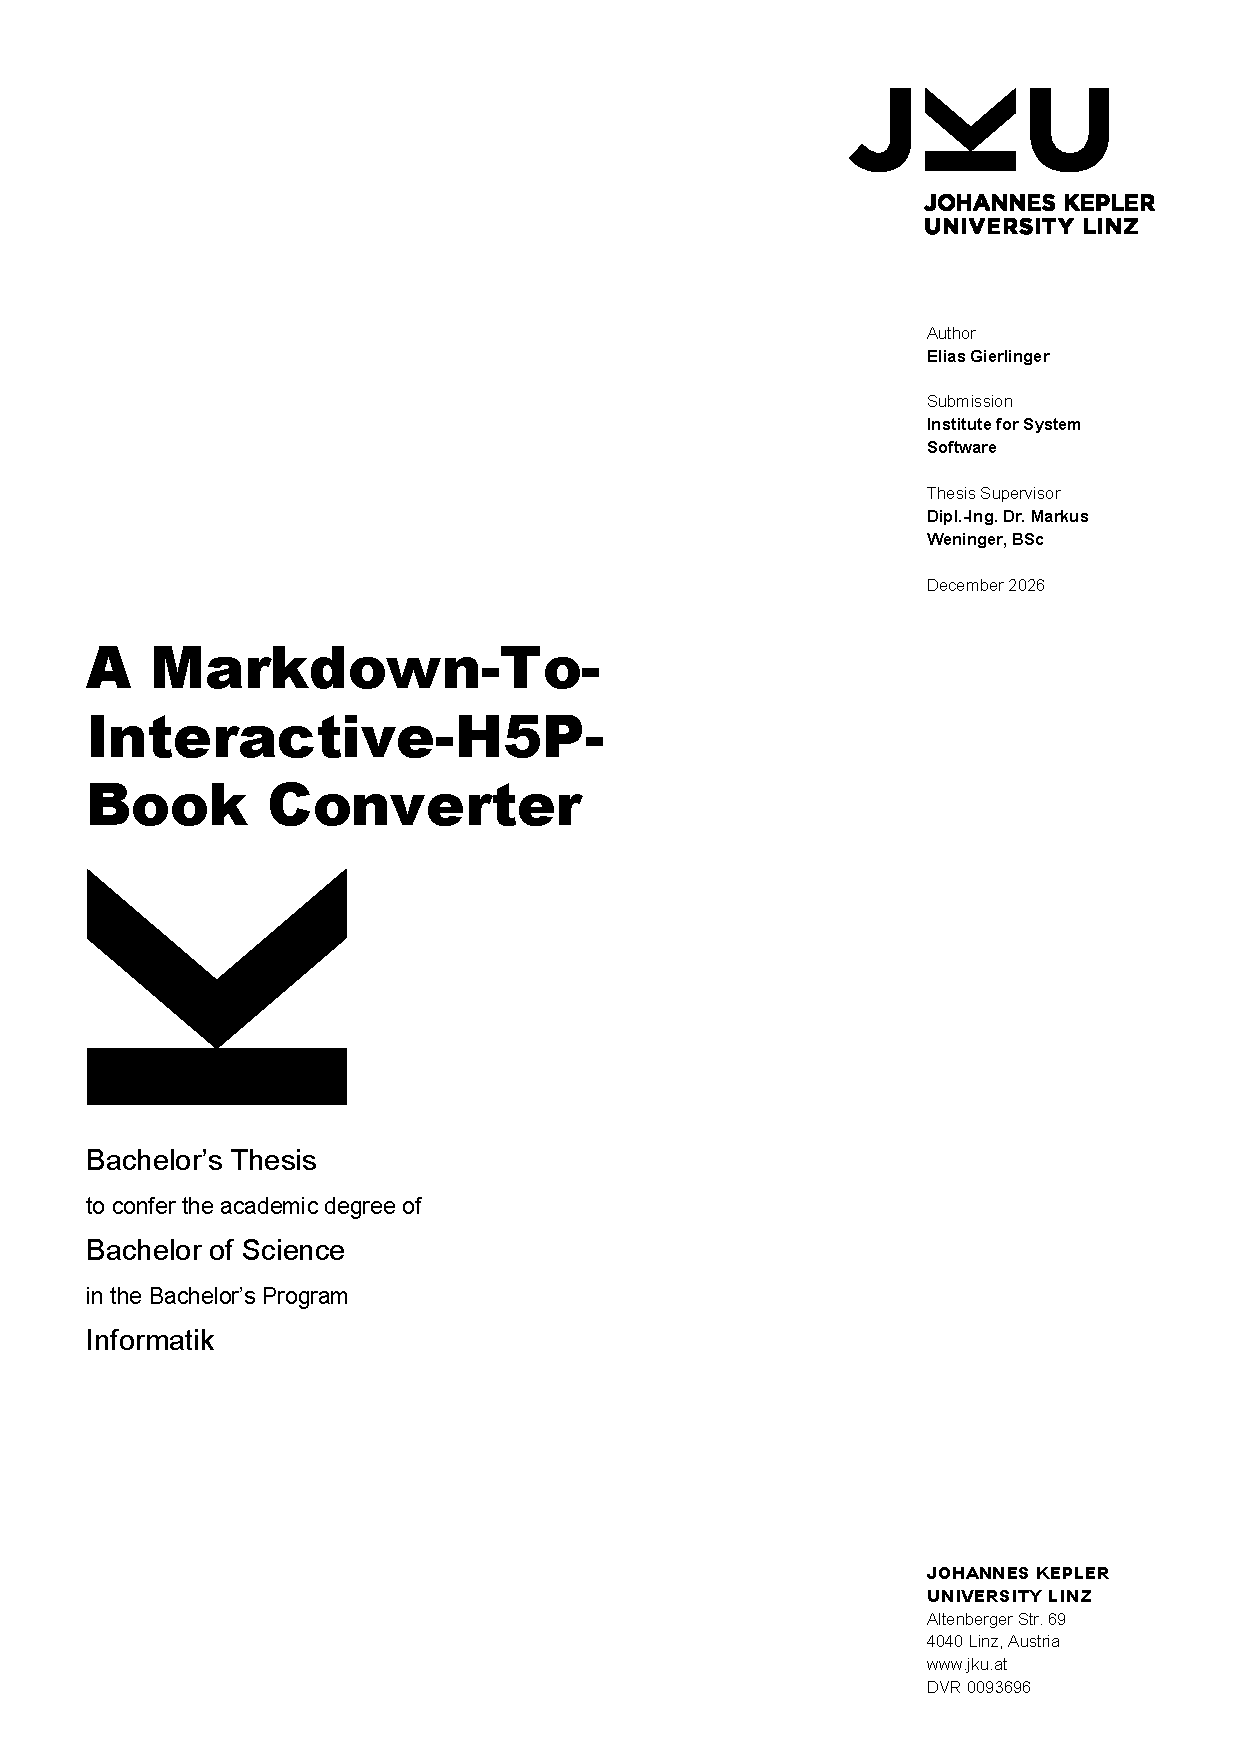
\includepdf{./pdfs/Cover.pdf}
\newpage
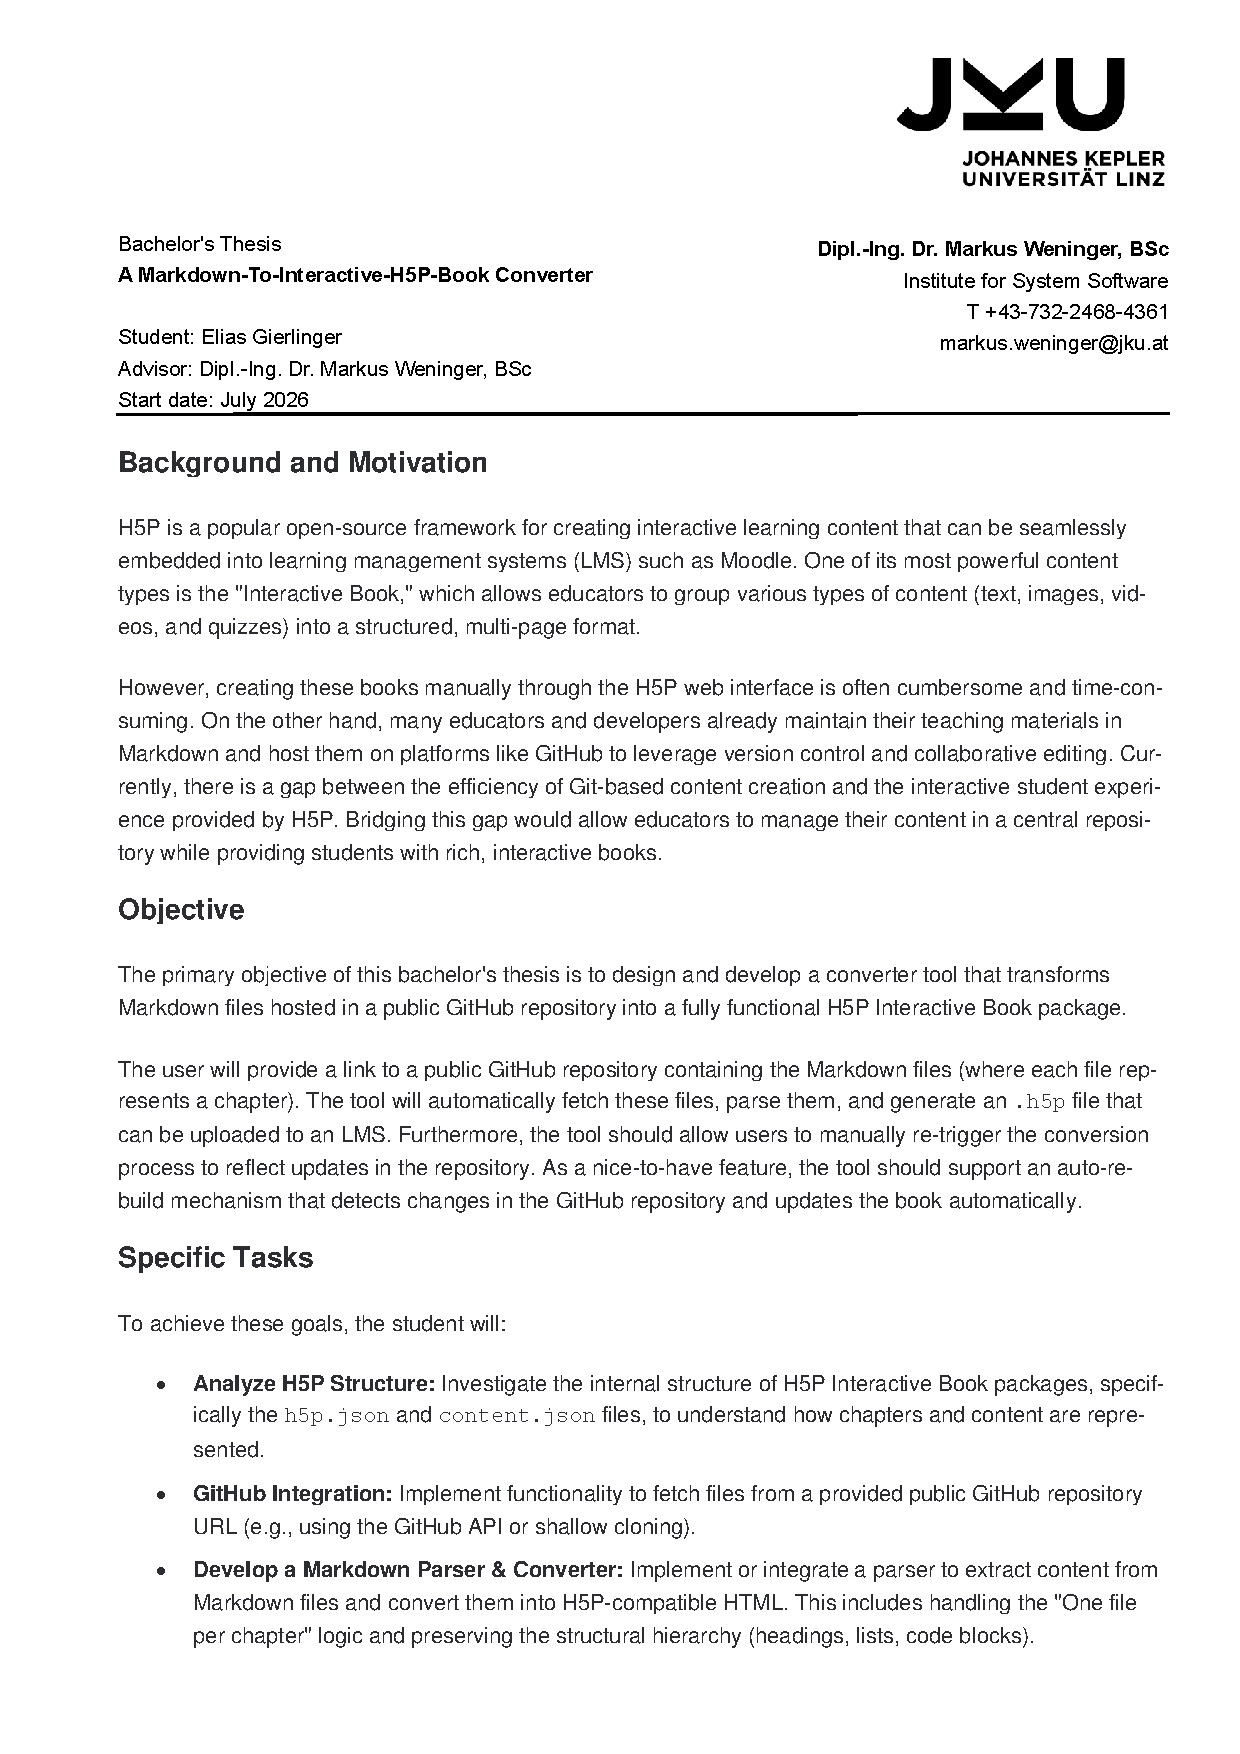
\includepdf[pages=-]{./pdfs/Topic.pdf}
\newpage

% ------------------------------------
% for abstract, kurzfassung, table of content we set the page number to roman numbers
\pagestyle{plain}
\renewcommand{\thepage}{\roman{page}}

\setcounter{page}{1}
\section*{Abstract}
\label{sec:abstract}
\addcontentsline{toc}{section}{\nameref{sec:abstract}}

Markdown's syntax is small and easily readable, which makes it well suited to writing documentation: being plain text, it can be opened and edited in a regular text editor, and its changes can easily be tracked by version control systems.
Using it for writing teaching materials is not ideal, though, not because Markdown itself falls short, but because the Moodle learning management system does not support it.
In Moodle, material can be authored as H5P packages in a browser-based editor.
This, however, means content written in Markdown is ported by hand, and the port is repeated every time the source changes.
H5P packages can be created for different content types, the most apt of which for representing Markdown files is Interactive Book: it represents content as chapters, each chapter made up of content blocks.
Those blocks come from a small set of content types with fixed nesting rules, so some Markdown constructs -- an image inside a table cell, for instance -- have no direct counterpart.
This thesis derives the limits of H5P's Interactive Book type and presents md2h5p, a converter that turns a folder of Markdown files into an H5P Interactive Book.
It renders each Markdown file into a chapter, finds alternatives for the Markdown constructs H5P does not support directly, and warns about constructs that can only be represented in a degraded form or not at all.
An extension adds single- and multiple-choice questions, written as Markdown fenced code blocks, and a
merge step folds a fresh conversion back into a package that has since been edited in the H5P editor.
Teachers can therefore keep authoring in Markdown, revise it after publication, and still
hand their students content the platform can embed.

\section*{Kurzfassung}
\label{sec:kurzfassung}
\addcontentsline{toc}{section}{\nameref{sec:kurzfassung}}

Die Syntax von Markdown ist klein und gut lesbar, weshalb sie sich zum Verfassen von
Dokumentation eignet: Da es sich um reinen Text handelt, kann er in jedem beliebigen Texteditor geöffnet und
bearbeitet werden, und Änderungen daran lassen sich mühelos von Versionsverwaltungssystemen
nachverfolgen.
Für das Schreiben von Lehrmaterial ist Markdown allerdings nur bedingt geeignet -- nicht, weil es
selbst zu kurz griffe, sondern weil das Lernmanagementsystem Moodle es nicht unterstützt.
In Moodle können Inhalte als H5P-Pakete in einem browserbasierten Editor erstellt werden.
Das bedeutet jedoch, dass in Markdown verfasstes Material von Hand portiert wird, und diese
Portierung wiederholt sich bei jeder Änderung der Quelle.
H5P-Pakete lassen sich für verschiedene Inhaltstypen erzeugen, von denen Interactive Book
Markdown-Dateien am ehesten gerecht wird: Dieser Typ gliedert Inhalte in Kapitel, wobei jedes
Kapitel aus einzelnen Inhaltsblöcken besteht.
Diese Blöcke stammen aus einer kleinen Auswahl von Inhaltstypen, die festlegen, was
worin verschachtelt werden darf.
Manche Markdown-Konstrukte -- etwa ein
Bild in einer Tabellenzelle -- haben daher keine unmittelbare Entsprechung.
Die vorliegende Arbeit lotet die Grenzen des H5P-Inhaltstyps Interactive Book aus und stellt
md2h5p vor, einen Konverter, der einen Ordner mit Markdown-Dateien in ein H5P Interactive
Book überführt.
Er übersetzt jede Markdown-Datei in ein Kapitel, findet für Markdown-Konstrukte, die H5P nicht
direkt unterstützt, geeignete Alternativen und gibt Warnungen für Markdown aus, das sich nur in
verminderter Form -- oder gar nicht -- darstellen lässt.
Eine Erweiterung ergänzt Single- und Multiple-Choice-Fragen, die als eingezäunte Codeblöcke in
Markdown geschrieben werden, und ein Merge-Schritt verbindet eine neue Konvertierung mit einem
Paket, das zwischenzeitlich im H5P-Editor bearbeitet wurde.
Lehrende können somit weiterhin in Markdown schreiben, ihr Material auch nach der Veröffentlichung
überarbeiten und ihren Studierenden dennoch Inhalte bereitstellen, die die Plattform einbetten kann.

\newpage

\setcounter{page}{2}
\renewcommand{\contentsname}{Table of Contents}
\tableofcontents
\label{sec:toc}
\newpage

% ------------------------------------
% starting from the introduction, we switch back to arabic numbers and start page numbering with 1 again
\renewcommand{\thepage}{\arabic{page}}
\setcounter{page}{1}

% it is up to you to have a separate .tex file per section or to put everything directly into this document
\section{Introduction}
\label{sec:introduction}

H5P is an open-source framework for interactive learning content.
An H5P content item is a
self-contained package that a learning platform embeds into its pages, and the Moodle learning
management system supports it out of the box: a teacher uploads a package, and students read it in
the browser as part of the course, with nothing to install and no external site to visit.
That
makes H5P attractive for course material of every kind, from a page of text to a set of
interactive questions.
Creating H5P content, however, means working in the platform's browser-based
editor.
Writing more than a few pages this way is slow, and
revising what has been written is slower still.

Markdown, on the other hand, is plain text with a handful of conventions for headings,
emphasis, lists, links, and code, so a chapter can be written in any text editor, kept in a Git
repository, reviewed as a diff, and shared without needing a particular program.
What Markdown lacks is a comfortable way to be read inside a course: a \code{.md} file attached to a Moodle page
is a download, and a student who opens it sees the raw syntax unless they have a viewer.
What is convenient to write is therefore not what is convenient to read.
The usual answer is to port the material by hand: open the H5P editor, paste and reformat each paragraph, upload
each image, rebuild each table.
This is tedious and must be repeated whenever the Markdown source changes to keep the source and the H5P copy in sync.

Among H5P's content types, Interactive Book is the one that best fits
a folder of Markdown files: it presents content as a sequence of chapters with a table of
contents, and each chapter is a list of content blocks such as text, images, and tables.
A folder
of Markdown files, one per chapter, maps onto it almost directly.

Almost, because the two formats do not line up completely, in both directions.
H5P has content
types for which Markdown has no syntax, such as quizzes or image hotspots.
Markdown, on the other
hand, permits structures that H5P refuses: an image inside a table cell is ordinary Markdown, but H5P table blocks may not contain images.
A converter therefore has to make compromises. The subject of this thesis is
which compromises are possible, which were chosen, and why.

The thesis makes five contributions.
(1) It works out what Moodle's H5P implementation actually
accepts in a text block, which HTML tags and which CSS declarations, by reading the sanitizer and
the content-type definitions, since the documentation does not say.
(2) For every
Markdown construct that has no direct counterpart, it presents a rendering strategy.
(3) It presents md2h5p, a
converter that turns a folder of Markdown files, a Git repository, or an upload into an Interactive
Book package and reports constructs it could only approximate as warnings.
(4) It adds a
small Markdown extension for single- and multiple-choice questions that leaves the source file
valid Markdown for every other tool.
(5) It adds a merge step that regenerates a book from changed
Markdown without losing what was added to the previous version in the H5P editor.

\newpage
\section{Background}
\label{sec:background}

The converter reads one format and writes another. Most of its design follows from what the
two allow.
This section introduces both Markdown and H5P.

\subsection{Markdown}
\label{sec:bg_markdown}

Markdown is a plain-text markup language: a document is an ordinary text file in which a few
conventions, such as \code{\#} for a heading, \code{*} for emphasis, and a leading \code{-} for a
list item, are interpreted by a renderer.
The original description of the
format~\cite{Gruber:Markdown} was a short, informal document with a reference implementation. It left many cases undefined, such as how list items nest or what happens to an emphasis marker
inside a word.
Each renderer resolved those cases on its own, so the same file rendered
differently from one tool to the next~\cite[Section 1.2]{CommonMark:Spec}.

\paragraph{CommonMark.}
The CommonMark specification~\cite{CommonMark:Spec} removed that ambiguity.
It defines the syntax precisely, with a test suite of several hundred examples. Most current
renderers implement it.
What CommonMark specifies is deliberately small: paragraphs, headings,
emphasis, lists, block quotes, code blocks, links, images, and raw HTML.
Everything else is left to
extensions.

\paragraph{Dialects and Extensions.}
Different platforms and editors thus use their own dialect, i.e., CommonMark
plus their own extensions.
GitHub Flavored Markdown~\cite{GitHub:GFM} adds tables,
strike\-through, and task lists. GitHub also supports footnotes and alerts outside that written
specification~\cite{GitHub:Writing}.
Obsidian~\cite{Obsidian:Links} also adds a link style called wiki links (\code{[[Target]]}), which points at another note by its name instead of
its path.
A third convention comes from the \TeX{} world: formulas between dollar signs, \code{\$x\$}
inline and \code{\$\$x\$\$} for display, which several editors and viewers render as \TeX{} would.
None of these are part of CommonMark, but a converter that accepts real-world documentation
must still accept them.

The converter described in this thesis uses commonmark-java~\cite{CommonMarkJava}, a Java implementation of
CommonMark, together with its extensions that correspond to GitHub Flavored Markdown.
Wiki links and dollar-delimited formulas are handled by two small parsers written for this thesis.
The parser turns Markdown into a tree of nodes:
a document holds block nodes such as paragraphs and lists, and those hold inline nodes such as text
runs, emphasis, and links.
Everything the converter does with a chapter starts from that tree.

\subsection{H5P}
\label{sec:bg_h5p}

H5P is a framework for interactive content.
A piece of content is a
\emph{package}, an \code{.h5p} file that platforms such as Moodle import, render, and edit.
The
package carries the content together with the code libraries the content needs to
run~\cite{H5P:Specification}, so a platform can install these libraries from the package.
Three aspects of H5P matter for this thesis: the structure of a package, the structure
of an Interactive Book, and what may go into a text block.

\begin{figure}[H]
	\centering
	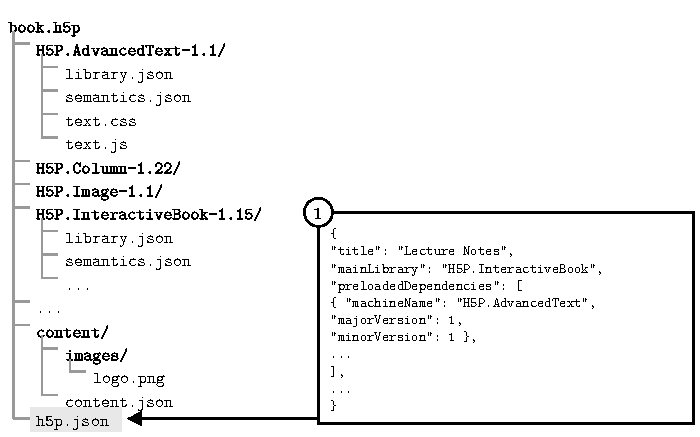
\includegraphics[width=0.9\columnwidth]{figures/package-h5pjson}
	\caption[The layout of a package and its \code{h5p.json}]{\label{fig:package_h5pjson}The layout
		of an \code{.h5p} package and the outline of its
		\code{h5p.json} \circled{1}.}
\end{figure}

\paragraph{Package Structure.}
An \code{.h5p} file is a ZIP archive with a fixed
layout~\cite{H5P:Specification,H5P:FileStructure}, shown in \autoref{fig:package_h5pjson}.
\code{h5p.json} \circled{1} at the root holds the metadata of the content, such as its title and content type, and lists under
\code{preloadedDependencies} every library the content needs~\cite{H5P:PackageDefinition}.

The libraries represent content types and may be bundled as folders named after the library and its version, such as \code{H5P.AdvancedText-1.1}~\cite{H5P:FileStructure}.
Each folder contains a \code{library.json} with its identity and dependencies~\cite{H5P:LibraryDefinition}, a
\code{semantics.json} describing its content model~\cite{H5P:Semantics}, and the
JavaScript and CSS that render it.
A package may, but does not have to, carry the
code of every library it uses~\cite{H5P:Specification}.
On import, the platform installs any libraries it lacks from the package.
If it cannot find them there, the import is refused~\cite{H5P:PhpLibrary}.

\begin{figure}[H]
	\centering
	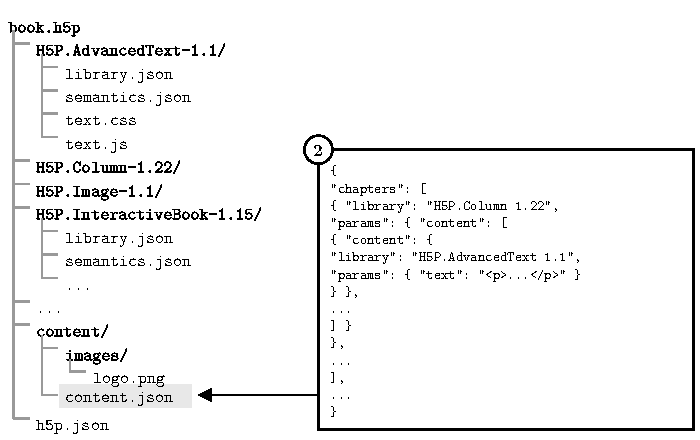
\includegraphics[width=0.9\columnwidth]{figures/package-contentjson}
	\caption[The \code{content.json} of a package]{\label{fig:package_contentjson}The same package
	with its \code{content/content.json} \circled{2} outlined: a list of chapters, each an
	\code{H5P.Column} whose \code{content} list holds the blocks of that chapter, each block
	naming its library and carrying its parameters.}
\end{figure}

The content itself is in \code{content/content.json} \circled{2}, a JSON document in which blocks are nested within other blocks, each providing its content type (\code{library}) and content (\code{params})
(\autoref{fig:package_contentjson}).
Media files referenced from it lie next to it under
\code{content/}, images for instance in \code{content/images}~\cite{H5P:Specification}.

\begin{figure}[H]
	\centering
	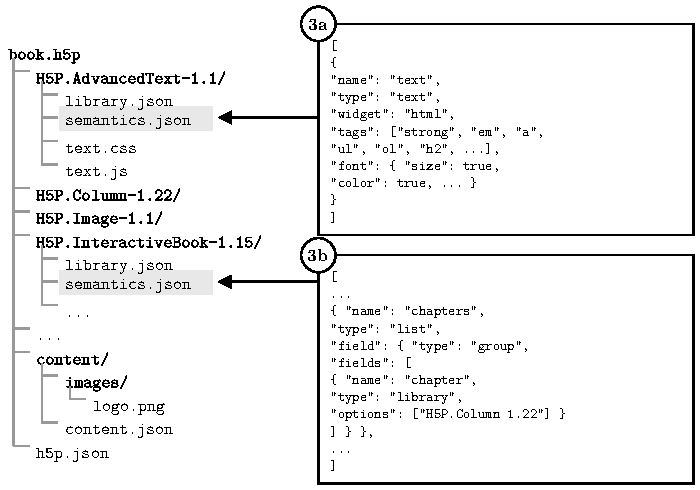
\includegraphics[width=0.9\columnwidth]{figures/package-semantics}
	\caption[The \code{semantics.json} of two libraries]{\label{fig:package_semantics}The same
	package with two \code{semantics.json} files outlined.
	\code{H5P.AdvancedText} \circled{3a} has one field of type \code{text}, with the HTML tags it
	permits and the font properties its editor offers.
	\code{H5P.InteractiveBook} \circled{3b} has a list of chapters, internally represented as \code{H5P.Column} blocks.}
\end{figure}

\code{semantics.json} merits a closer look, because the restrictions
discussed in this thesis stem from it~\cite{H5P:Semantics}.
It is the schema of a content type and describes how the content must be structured and which elements it consists of (\autoref{fig:package_semantics}).
For example, AdvancedText \circled{3a} consists of no more than a text field limited in the set of allowed HTML tags and font styling.
Interactive Book \circled{3b}, by contrast, comprises a list of Column blocks, appropriately called chapters.
For such nesting, a content type must specify the exact versions of the content types it references, tightly coupling the versions of the libraries in a package.

\begin{figure}[H]
	\centering
	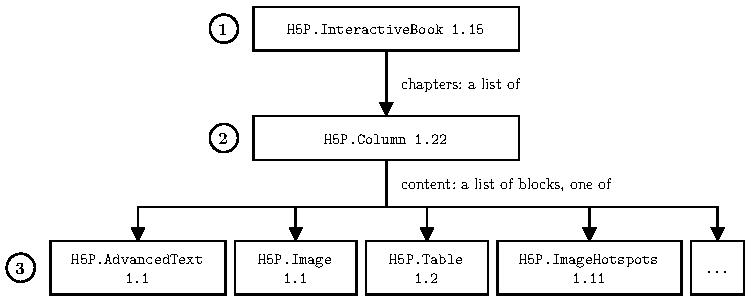
\includegraphics[width=0.9\columnwidth]{figures/book-model}
	\caption[The content model of an Interactive Book]{\label{fig:book_model}The content model of
	an Interactive Book. The book \circled{1} holds a list of chapters, each an \code{H5P.Column}
	\circled{2}, and a column holds a list of blocks \circled{3}, each an instance of one of the
	content types its \code{semantics.json} names.}
\end{figure}

\paragraph{Interactive Book.}
H5P offers many content types, from simple types like AdvancedText and Image to more complicated types such as Course Presentation or Interactive Book that are built from other types.
Interactive Book~\cite{H5P:InteractiveBook} is the one that resembles a multi-chapter document; its viewer shows a table of contents in a sidebar and tracks
reading progress.
In its \code{content.json}, it consists of a list of chapters (\autoref{fig:book_model}),
each chapter being an \code{H5P.Column} \circled{2} and a column being a vertically arranged list of content blocks \circled{3},
each of which is an instance of one of the allowed content types.
The blocks the converter writes are \code{H5P.AdvancedText} for text,
called a \emph{Text block} for brevity, \code{H5P.Image} for images, \code{H5P.Table} for
tables, \code{H5P.Row} with \code{H5P.RowColumn} for a side-by-side layout, and
\code{H5P.SingleChoiceSet} and \code{H5P.MultiChoice} for questions.

\paragraph{Text Blocks.}
A Text block carries one HTML string. This is where the central
constraint of the thesis lies.
Before being shown to the user, a sanitizer runs over it and keeps only the tags the block's \code{semantics.json} permits,
plus a few that are always allowed; a disallowed tag is removed, but its text content is kept.
The remaining HTML tags are further stripped of any illegal CSS styling inside their \code{style} attributes.
Which CSS declarations are allowed is defined in a fixed list specific to each platform (Moodle in this thesis) that the library's
\code{font} declaration in \code{semantics.json} can extend.
Since no stylesheet can be shipped with the content, those
inline styles are the only way to make anything look different from the default.
For now, it is enough to know that \code{img} and \code{table} are among the tags a Text block does not accept: to represent them, the separate Image and Table content types must be used.

\newpage
\section{Usage}
\label{sec:usage}

Before examining the conversion in detail, this section presents md2h5p from the user's perspective:
Markdown files are converted into an Interactive Book package, accompanied by conversion warnings.

md2h5p can be used in two ways.
As a command-line program, it converts a folder on the
local machine or a public Git repository.
Alternatively, it can run as a web application that accepts a
repository URL or uploaded files in the browser.

\paragraph{Command Line.}
A local conversion is one command that names the folder holding the
chapters:

\begin{lstlisting}
md2h5p convert --folder notes/
\end{lstlisting}

The folder is expected to hold one Markdown file per chapter, in the order given by a leading number
in the file name (\code{1\_intro.md}, \code{2\_setup.md}, \ldots), together with the images those
files reference.
The package is written to the directory the command was run from, named after the
folder unless overridden by \code{--output}.
The folder name also serves as the book's title if no \code{--title} is specified.
To convert a repository instead, \code{--repo} takes its URL
and, if the chapters are not at the root, \code{--subfolder} takes the path inside it.
A further option,
\code{--merge-with}, takes a package that was previously generated and has since been edited in the H5P editor.
The conversion then inserts what was added there into the new package.
Warnings are printed to the console after the conversion.

\begin{figure}[H]
	\centering
	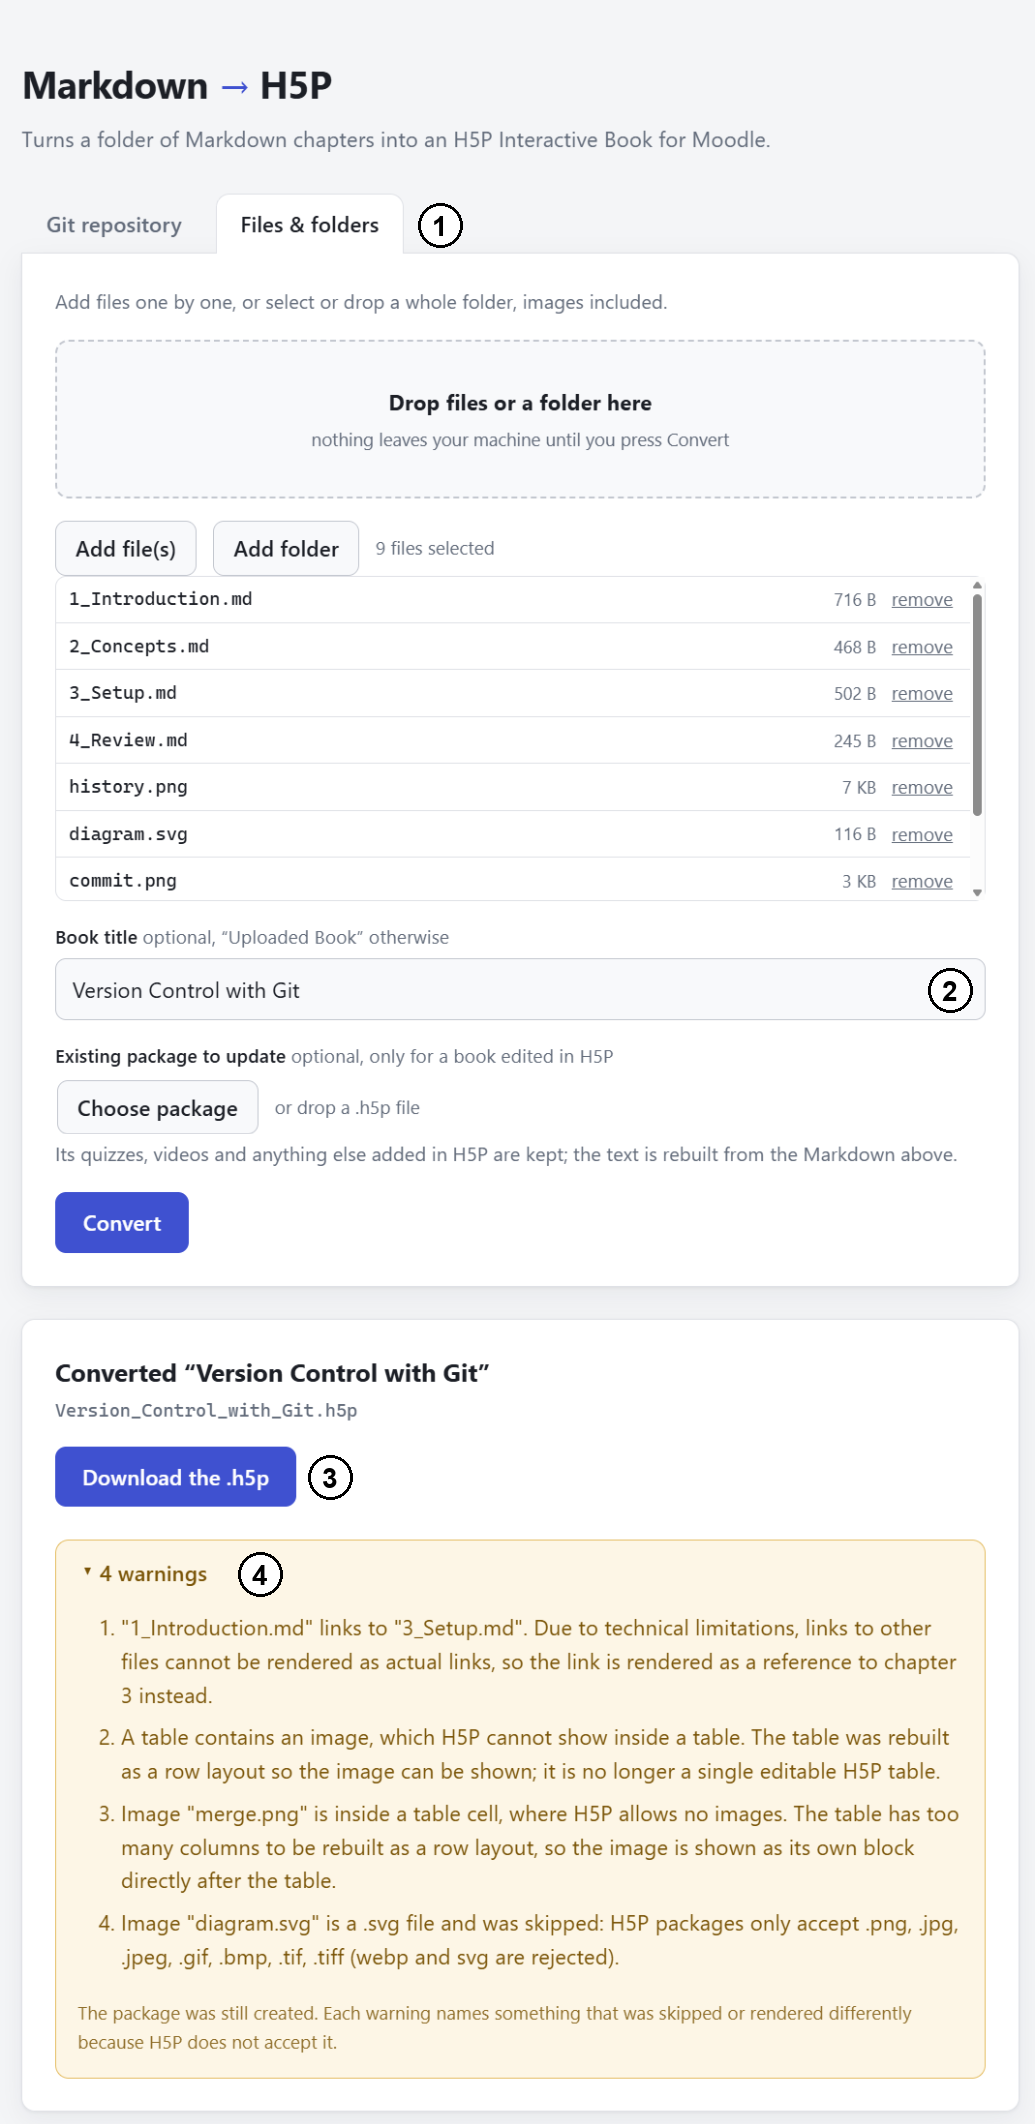
\includegraphics[width=0.68\columnwidth]{figures/screenshots/usage-web}
	\caption[The web interface after a conversion]{\label{fig:usage_web}The web interface after a conversion.
	The warnings \circled{4}
		are part of the result and appear beside the download \circled{3}.}
\end{figure}

\paragraph{Web Interface.}
The server is started with \code{md2h5p serve} and shows one page.
It has two tabs, one for converting a repository and one for uploaded files.
The web UI offers the same configuration options as the CLI: an optional title field, a subfolder field, and a file input for an existing \code{.h5p} package to merge into the new package.
The user starts the conversion by pressing \emph{Convert}.
Once the server has finished, the page shows a result panel with the title, the file name, a download
button, and the list of warnings.
\autoref{fig:usage_web} shows the page after a conversion.

\begin{figure}[H]
	\centering
	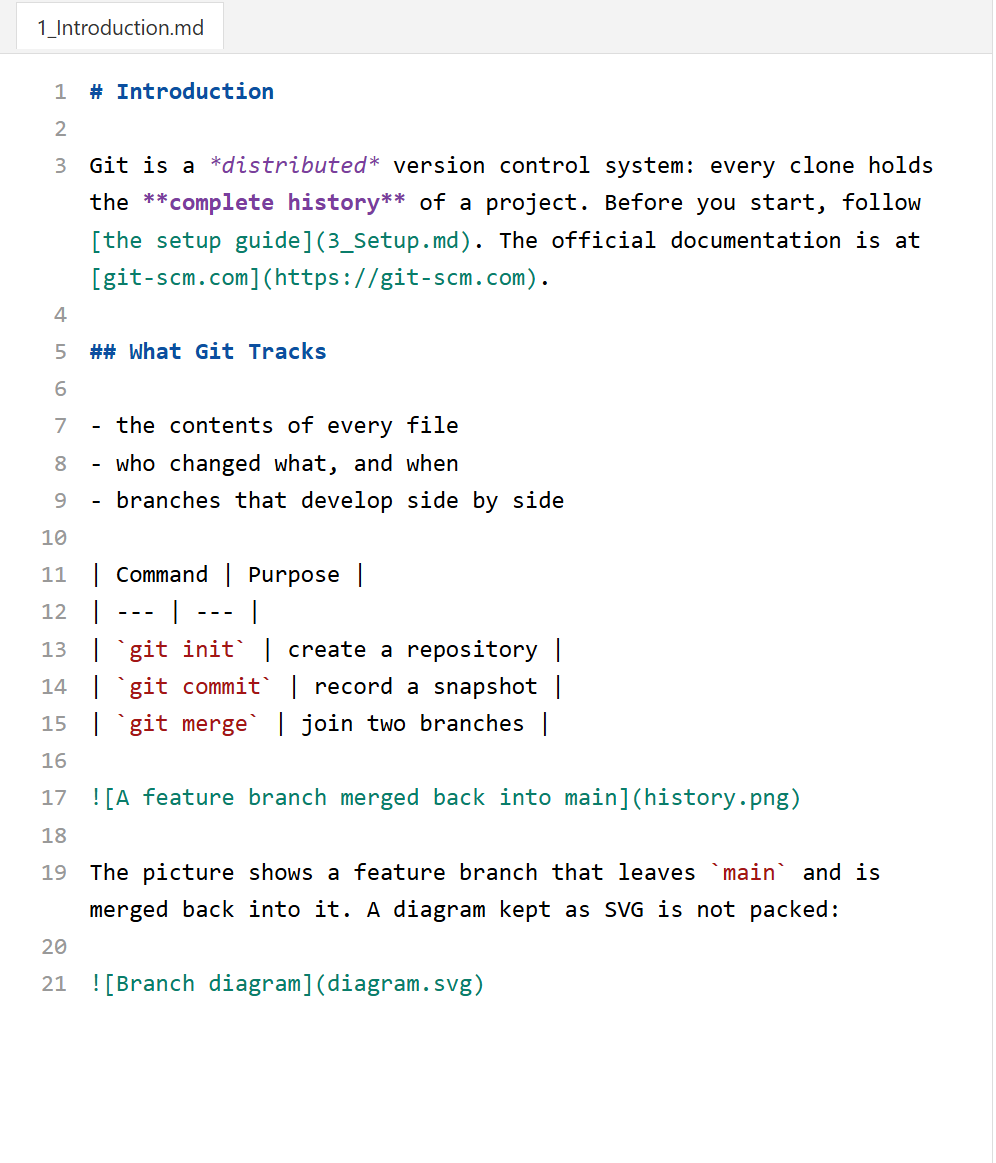
\includegraphics[width=0.485\columnwidth]{figures/screenshots/usage-result-editor}\hfill
	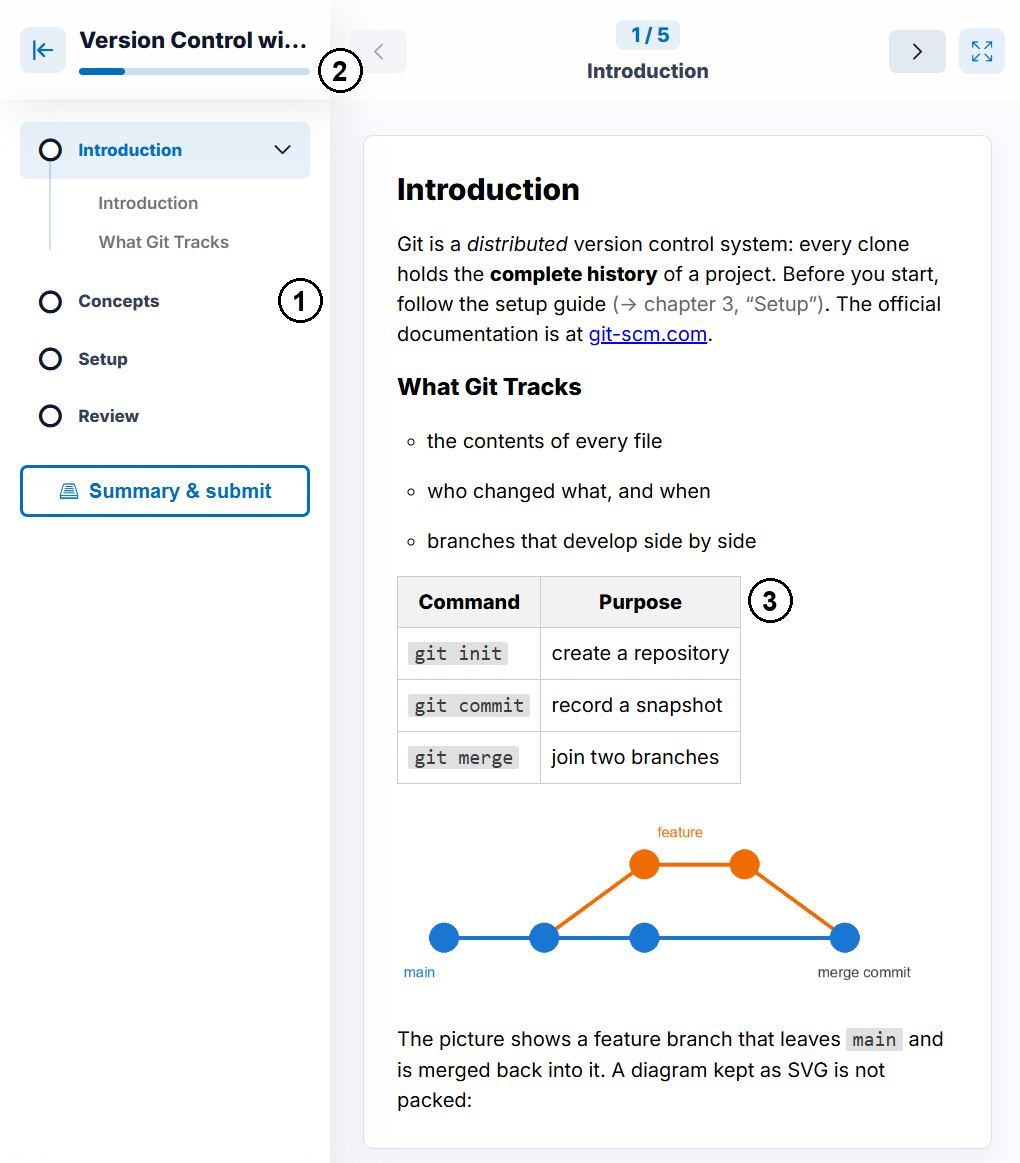
\includegraphics[width=0.485\columnwidth]{figures/screenshots/usage-result-moodle}
	\caption[A chapter in Markdown and in Moodle]{\label{fig:usage_result}A chapter as written in Markdown and as read in Moodle.
	Every
		file has become a chapter with an entry in the sidebar \circled{1}, the book tracks progress
		\circled{2}, and the table \circled{3} carries its borders although the target has no
		stylesheet for it.}
\end{figure}

\paragraph{The Result.}
\autoref{fig:usage_result} shows a chapter as it was written
and as it is read in Moodle.
On the left is the Markdown file in an editor; on the right, the same chapter in
Moodle.
Each file has become a chapter with the file's first heading as its title. The
chapters appear in the sidebar as a table of contents, with every heading of a chapter listed
below it.
The book also keeps a progress indicator across chapters.
To move between them, the reader uses the sidebar or the next and previous buttons.
The text, its formatting, the table, and the image on
the right are what the Markdown specified, rendered in the form the platform accepts.

\newpage
\section{Overview}
\label{sec:overview}

\begin{figure}[H]
	\centering
	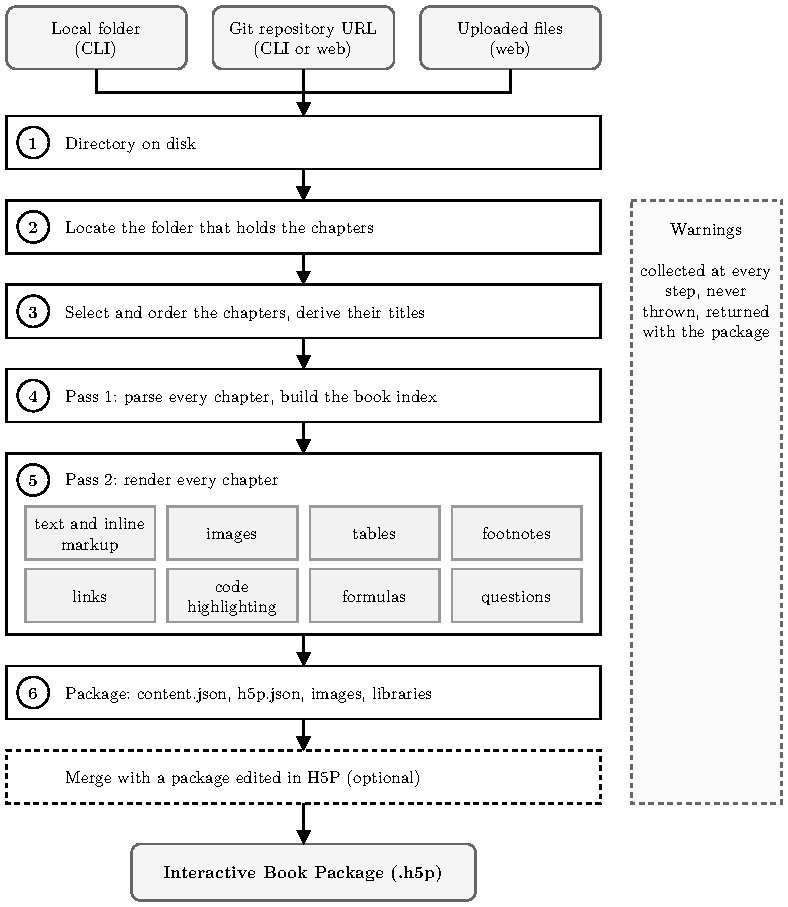
\includegraphics[width=0.92\columnwidth]{figures/pipeline}
	\caption[The conversion pipeline]{\label{fig:pipeline}The conversion pipeline.
	All three input modes produce a directory
		on disk \circled{1}; the folder holding the chapters is located \circled{2}, the chapters are
		selected and ordered \circled{3}, every file is parsed and indexed \circled{4}, then rendered
		\circled{5}, and the result is packaged with the libraries it needs \circled{6}.
		Warnings are
		collected at every step and returned together with the package.}
\end{figure}

The usage examples showed the converter as a black box.
md2h5p is implemented in Kotlin and runs on the Java Virtual Machine (JVM).
This section describes its scope, the steps of a conversion, the three input modes, how errors are
handled, and how an already edited package is updated.
\autoref{fig:pipeline} shows the pipeline; the text refers to its numbered steps.

\paragraph{Scope.}
The converter takes a folder of Markdown files, one per chapter, and produces
an Interactive Book package for Moodle.
It carries over the structure of the text (headings, paragraphs, lists, block quotes), inline
formatting, images, tables, links, footnotes, and code blocks.
It also renders three constructs that go beyond plain Markdown:
highlighted code, formulas, and simple quizzes.
It does not create new H5P content types and does not upload anything to Moodle.
Where Interactive Book cannot represent a construct directly, the converter produces the closest
supported approximation.
Warnings identify input that requires the author's attention.

\paragraph{Pipeline.}
A conversion starts from a directory on disk \circled{1}.
The directory may hold more than the chapters, a whole repository for instance, so the first step
is to find the folder with the Markdown files \circled{2}.
From that folder, they are selected, put into chapter order, and given titles
\circled{3}.
The chapters are then processed in two passes.
The first pass \circled{4} parses every file and records each chapter's title, file name, package identifier,
and heading anchors in an index of the whole book.
The second pass \circled{5} renders each chapter into content blocks, with separate renderers for
the more complex constructs.
Images are resolved and copied during this pass.
Finally, the generated \code{content.json} and \code{h5p.json} are zipped together with the images
and the H5P libraries the book depends on \circled{6}.

This separation into two passes is needed for links.
A link in chapter~2 may point at chapter~5. To render it, the converter has to know whether that
chapter exists, what it is called, and which identifier it carries.
Since a link may point forwards, every chapter has to be parsed before the first one is rendered.

\paragraph{Input Modes.}
The content arrives in one of three ways: a folder on the local machine, a Git repository that is
shallow-cloned, or files uploaded through the browser.
All three end up as a directory on disk \circled{1}, so one pipeline serves every mode.
After that point, the modes differ only in how far the converter trusts the content.
A local folder belongs to the person running the converter, so its Markdown may reference an image
anywhere on that machine.
A clone or an upload, by contrast, was written by somebody else and may only reference files inside its own
directory.

\paragraph{Warnings.}
\label{sec:ov_warnings}
The pipeline does not abort on bad input.
A missing image, a path that leaves the allowed directory, an image format the platform rejects, a
table too wide to be rebuilt around an image, or a quiz without a correct answer each results in a
\emph{warning} and a defined fallback.
The book is still produced, so a single unsupported image in one chapter does not
cost the entire conversion.
The warnings are collected at every step and returned together with the package.
Together, these warnings list what the author has to fix or accept.

\paragraph{Updating an Edited Package.}
Interactive Book can hold content that Markdown cannot express, such as a video or an image with
hotspots, which a teacher adds in the H5P editor after the conversion.
If the Markdown changes afterward, a new conversion would produce a package without these
additions.
The converter therefore accepts the edited package as a second input and merges it with the new
conversion.
The text is rebuilt from the Markdown, while every block added in the editor is kept and placed after
the paragraph it followed before.
The merge is a post-processing step on two finished packages and does not change the pipeline above.
It has two limitations: an edit made in the editor to text that came from Markdown is overwritten,
and when paragraphs are reordered in the Markdown, an added block may end up under the wrong one.
Both cases are reported as warnings.

\newpage

% --- main chapters ---
\section{Chapters and Referenced Files}
\label{sec:files}

The converter is given a directory.
It may be a folder that contains only the chapters, or a whole repository with a README, several
documentation folders, and an archive of old notes, any of which may contain Markdown files.
Before anything is rendered, the converter must decide which files become chapters, in which order,
and under which titles.
It must also determine how referenced files get into the package.

\subsection{Chapter Folder, Order, and Titles}
\label{sec:in_folder}

\paragraph{Locating the Chapter Folder.}
In a repository, the chapters are rarely at the root.
A repository typically holds a README at the top, the chapters somewhere below it, and often other
folders with Markdown files that are not part of the book.
Instead of requiring the user to always name the folder, the converter locates it on its own.
It reports which other folders it could have chosen, so that the user can convert again with an
explicit choice if the guess was wrong.

\begin{figure}[H]
	\centering
	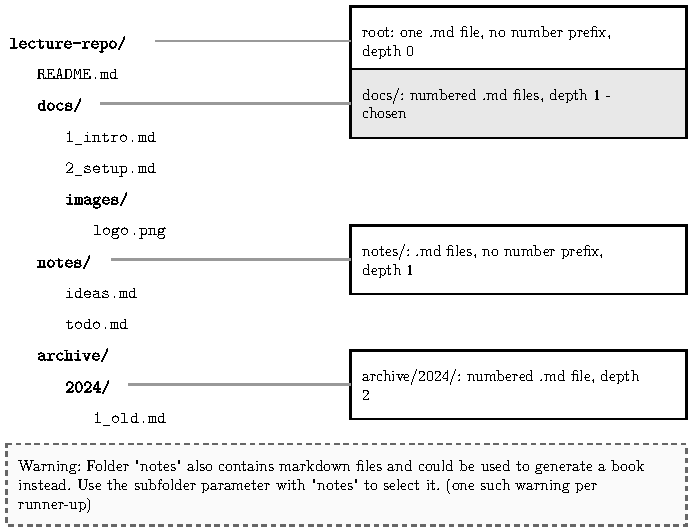
\includegraphics[width=0.9\columnwidth]{figures/chapter-folder}
	\caption[Locating the chapter folder]{\label{fig:chapter_folder}Locating the chapter folder in a repository with four
		folders that directly contain Markdown.
		The root and \code{notes/}
		have no numbered file; \code{archive/2024/} has one but lies deeper than
		\code{docs/}, which is chosen.
		Each runner-up produces one warning naming the
		parameter that would select it instead.}
\end{figure}

Only folders that contain Markdown files are candidates.
Among them, the converter prefers
a folder containing a Markdown file with a leading number in its name, since this is
the chapter-ordering convention described below;
the shallowest folder, since archives and drafts tend to lie deeper than the chapters;
and, on a tie, the alphabetically first.
Every candidate not chosen is named in a warning, together with the subfolder parameter
that would select it.
\autoref{fig:chapter_folder} shows a repository with four candidates and the resulting choice.
Alternatively, an explicit subfolder parameter skips the search.
It must lie within the input directory; if it does not exist, the search still runs, and a
warning is issued.

\paragraph{Chapter Order.}
\label{sec:in_order}
Inside the chosen folder, every file with the extension \code{.md} becomes a chapter.
Subfolders are not searched, so that a folder of images or appendices next to the chapters does not
add chapters.
Files whose name starts with a digit come first, sorted by the numeric (rather than alphabetic) value of that prefix,
so \code{10\_summary.md} follows \code{2\_setup.md}.
Files without a number follow in alphabetical order.
If a folder mixes the two conventions, a warning names the unnumbered files, but none of them is
dropped, since silently dropping a chapter would lose content.
The number prefix may be followed by a dot, a parenthesis, a hyphen, an underscore, or spaces, all of
which are stripped.

\paragraph{Chapter Titles.}
The title of a chapter is the text of its first heading, if the file starts with one.
YAML front matter at the top of the file does not count as content, so a heading right after it
still counts as first.
Otherwise, the title is the file name without the number prefix and with underscores replaced by
spaces, so \code{3\_getting\_started.md} becomes ``getting started''.
A heading that became the title is also kept in the chapter body.
The sidebar entry that shows the title is often truncated, and a chapter that opens without a
visible heading reads worse than one whose title appears twice.

\subsection{Path Resolution and Trust Boundaries}
\label{sec:files_paths}


In practice, the files referenced by a chapter are images, and every reference is a path that the converter has to resolve to a file.
Unlike chapter discovery, path resolution depends on the input mode, because a path can point anywhere.
A Markdown file containing \code{![](../../../etc/}\allowbreak\code{passwd)} makes no sense as documentation.
A server that resolves this path and packs the file into a downloadable archive, however, leaks a
file from its own disk to whoever submitted the repository.
This is the path traversal weakness cataloged as CWE-22~\cite{MITRE:CWE22}, which the converter has
to prevent on the server without breaking the normal case on the desktop.

\paragraph{Trust Boundaries.}
A clone or an upload was written by somebody other than the operator, so its content must not
reach anything outside the directory it was placed in.
A local folder, by contrast, is converted by the person running the command, who already has full access to the
file system.
Restricting it would protect nobody and would break notes that reference an image elsewhere on the
disk, for instance in a shared assets folder or on another drive.
The policy therefore depends on the input mode: a local folder is unrestricted, while a clone or an
upload is confined to its directory.
The same trust boundary applies to downloading remote images.

\paragraph{Resolution Order.}
A referenced path is resolved in four steps.
\circled{1} It is interpreted relative to the directory of the Markdown file that contains it, and
if a file exists there, that file is used.
\circled{2} Otherwise, it is interpreted as an absolute path.
The relative interpretation comes first because a repository-style path such as
\code{/images/logo.png} would otherwise be read as absolute on Unix systems and fail.
\circled{3} The result is canonicalized, applying every \code{..} and resolving symbolic links,
so that the following check cannot be bypassed.
\circled{4} For a clone or an upload, the canonical path has to lie inside the input directory;
otherwise the reference is rejected.
A rejected path, a nonexistent file, and a path that cannot be canonicalized at all
each produce a warning; the image is omitted.

\paragraph{Uploads and Submitted Packages.}
Two further kinds of names come from outside and are checked in the same way.
In a multipart upload, the client names every file, and a name such as \code{../../x.md} would
otherwise place the file outside the staging directory. Such a file is rejected.
A package submitted for merging is a ZIP archive whose entry names are chosen
by the client as well, and an entry that is absolute or leaves its directory is rejected for the same
reason.
The merge reads the archive without unpacking it, which avoids most of this problem in the first
place.

\subsection{Images}
\label{sec:sec_images}

Images are referenced in nearly every chapter. They have to be copied into the package because
H5P has no notion of an image stored elsewhere.
This raises three questions: what an image is called inside the package, which files may be
included, and how to handle images that are not local files.

\paragraph{Naming in a Flat Folder.}
All images of a book end up in the single folder \code{content/images} of the package, regardless of
how the author's folders were organized.
The file name alone is not unique: two chapters that both reference a file named
\code{logo.png} in different folders would map onto the same entry, and a duplicate entry would abort the creation of the
archive.
The converter therefore appends the first twelve bytes of the image's SHA-256 hash to its sanitized file name,
followed by the extension, for instance \code{logo-3f9a2c17b0e4d5a6c1f83a23.png}.
Collisions between different files are thus extremely unlikely, and repeated references to the same
image share a single stored copy.
Moreover, the packed name does not depend on where the file was located on the author's machine.


\paragraph{Accepted Formats.}
Moodle validates every file in a package against a list of allowed extensions, and a package with a
single file outside that list is rejected as a
whole\footnote{\raggedright \code{validateContentFiles} in \code{h5p.classes.php}, lines 4420--4454, against
the list \code{H5PCore::\$defaultContentWhitelist} at line 2118; Moodle passes the list through
unchanged (\code{h5p/classes/framework.php}, line 698).}~\cite{H5P:PhpLibrary}.
For images, the list contains \code{png}, \code{jpg}, \code{jpeg}, \code{gif}, \code{bmp},
\code{tif}, and \code{tiff}.
Any other image, such as \code{webp}, \code{svg}, or a file with no extension, is therefore omitted from the
package with a warning.
If it were included, Moodle would reject the entire book.
Only the extension is checked, not the file content. Unsupported formats are not converted,
since this would add an image-processing dependency for a problem that belongs in the source
document.
In practice, \code{svg} is the most common case, because diagrams are often kept in that format;
the author has to export them as PNG.

\paragraph{Remote Images.}
Markdown allows an image to be referenced by URL, which is common in notes written in a wiki or an
issue tracker.
Since the package cannot reference anything outside itself, the converter downloads the image at
conversion time and treats it like a local file, with the same extension check and naming.
Leaving the reference in the markup is not an option, because the sanitizer removes every
\code{img} tag and only the alternative text would remain.
A reference counts as remote if it starts with a scheme of at least two letters, so that a Windows
path such as \code{C:/notes/logo.png} is not mistaken for a URL.
The content type of the response is checked as well, so that an HTML error page returned with
status 200 is not packed as an image.
If the URL has no extension, that same content type determines the file type.

On the web server, the download is a request to an address chosen by a stranger.
A request to \code{http://127.0.0.1:8080/} or to a cloud provider's metadata endpoint would be made
from inside the server, and the response would be packed into a book anyone can download.
This is known as server-side request forgery.
The download is therefore limited in four ways:
a timeout;
a size limit of 20 MB, enforced while reading instead of relying on the \code{Content-Length}
header;
a refusal of any loopback, link-local, site-local, unique-local, or multicast address;
and redirects, at most three, checked as well since the target of a redirect may also be a private
address.
As with paths, the address check applies to a clone or an upload but not to a local folder.
Somebody converting their own notes can open these addresses in a browser anyway, and notes that
reference a wiki or a documentation server on \code{localhost} are a legitimate case.

\paragraph{Embedded Images.}
A \code{data:} URL contains the image itself, base64- or percent-encoded, and some Markdown editors
write one when an image is pasted into a document.
Such a URL is decoded instead of downloaded, its media type takes the role of the content type, and
the result is treated like a local file.

Every failure described in this section produces a warning, but the book is still produced.

\newpage
\section{Rendering Markdown Text}
\label{sec:markup}

Once the chapters are known, each of them has to become a list of content blocks, most of which are
Text blocks carrying HTML.
This section covers the constructs that can be expressed as markup inside a Text block: text,
headings, lists, emphasis, block quotes, and code.
Images, tables, and the constructs that enclose them require separate content blocks.

Every decision in this section depends on \autoref{tab:allowed}, which lists what survives the
sanitizer in the two libraries the converter writes text into.
The upper half lists, per tag, whether a Text block and a Table block keep it and whether it may
carry a \code{style} attribute; the lower half lists which declarations inside that attribute
are kept.
The table was derived from the sanitizer implementation and the \code{semantics.json} of both
libraries\footnote{\raggedright Tags: \code{validateText} in
\code{h5p.classes.php}, lines 4303--4327, starting from the library's \code{tags} array and
always adding \code{div}, \code{span}, \code{p}, and \code{br}; styleable tags:
\code{\$allowed\_styleable\_tags}, lines 4201--4214; declarations: \code{\$stylePatterns}, lines
4330--4376, unlocked per library by its \code{font} block and by \code{table} being among its
tags.}~\cite{H5P:PhpLibrary}.
Two of its properties shape the rest of the conversion.
First, the rules differ per library: \code{table} is allowed in a Table block but not in a Text
block; \code{border} and \code{padding} exist only for libraries that permit \code{table}.
Second, the rules cannot be changed.
A library's \code{semantics.json} is part of the package, but the platform keeps the copy it already
has installed, so a modified one would be ignored.

\begin{table}[H]
	\centering
	\small
	\begin{tabular}{@{}>{\raggedright\arraybackslash}p{0.45\columnwidth}cc>{\raggedright\arraybackslash}p{0.24\columnwidth}@{}}
		\toprule
		\textbf{Tag} & \textbf{AdvancedText} & \textbf{Table} & \textbf{Styleable} \\
		\midrule
		\code{div}, \code{span}, \code{p} & \tyes & \tyes & \tyes \\
		\code{br}, \code{strong}, \code{em}, \code{del}, \code{s}, \code{a}, \code{code} & \tyes & \tyes & \tno \\
		\code{h2}, \code{h3}, \code{li} & \tyes & \tno & \tyes \\
		\code{ul}, \code{ol}, \code{hr}, \code{pre} & \tyes & \tno & \tno \\
		\code{table}, \code{td}, \code{th}, \code{col}, \code{figure} & \tno & \tyes & \tyes \\
		\code{tr}, \code{thead}, \code{tbody}, \code{tfoot}, \code{colgroup}, \code{figcaption} & \tno & \tyes & \tno \\
		\midrule\midrule
		\textbf{Style Declaration} & \textbf{AdvancedText} & \textbf{Table} & \textbf{Unlocked by} \\
		\midrule
		\code{text-align} & \tyes & \tyes & every text \\
		\code{color} & \tyes & \tyes & \code{font} semantics \\
		\code{font-size} & \tyes & \tno & \code{font} semantics \\
		\code{background-color} & \tyes & \tyes & \code{font} semantics; table group \\
		\code{border}, \code{border-style}, \code{border-width}, \code{border-color}, \code{border-collapse}, \code{padding}, \code{vertical-align}, \code{width}, \code{height}, \code{float} & \tno & \tyes & table group \\
		\bottomrule
	\end{tabular}
	\caption[What survives H5P's sanitizer in a Text block and a Table block]{\label{tab:allowed}What survives H5P's sanitizer in the two libraries the converter
		writes text into.
		Styleable says whether a \code{style} attribute is kept on the tag at
		all; a declaration inside it then has to pass the lower half, where table group is the
		set unlocked for any library whose semantics permit \code{table}.
		Anything not listed is
		dropped silently.
		Derived from the sanitizer implementation and the libraries'
		\code{semantics.json}, not from documentation.}
\end{table}

\subsection{Document Traversal}
\label{sec:mk_visitor}

commonmark-java includes an HTML renderer, but the converter does not use it.
The sanitizer removes a tag it does not permit and keeps its text, so a \code{blockquote} produced by
the renderer would silently turn into an ordinary paragraph.
Such a loss is only noticed by comparing the source with the book.
Post-processing the renderer's output would mean parsing the HTML again and rewriting every tag the
platform does not accept.
Moreover, the mapping is not one tag to another: a block quote becomes a \code{div} with a label and
a background.
The converter therefore renders the node tree itself and only emits markup that survives, so
every deviation from the Markdown is intentional.

\begin{figure}[H]
	\centering
	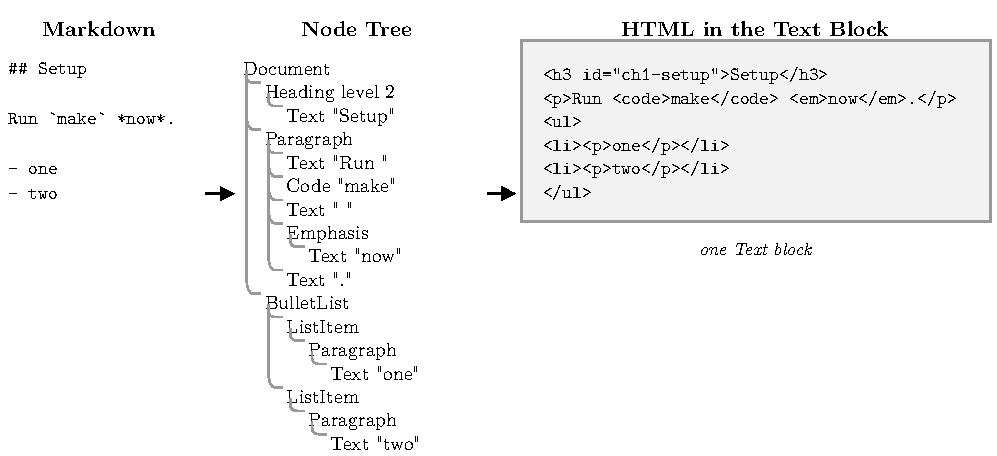
\includegraphics[width=\columnwidth]{figures/render-tree}
	\caption[From Markdown to the node tree to HTML]{\label{fig:render_tree}A Markdown fragment, the node tree the parser produces, and the
		HTML the visitor emits.
		The heading, emphasis, and list
		each map onto a permitted tag; the whole fragment lands in a single Text block.}
\end{figure}

The parser produces a tree in which a document holds block nodes, blocks hold inline nodes, and
every node type is a class.
To traverse this tree, the converter uses a visitor with one method per node type.
Nearly every method opens a tag, renders the children, and closes the tag.
For example, \autoref{lst:emphasis_visitor} shows how the emphasis visitor wraps its children in
\code{em}.

\begin{lstlisting}[language=Kotlin,
caption={[The emphasis visitor]The emphasis visitor.},label={lst:emphasis_visitor}]
override fun visit(emphasis: Emphasis) {
    html.pushTag("em")
    visitChildren(emphasis)
    html.popTag()
}
\end{lstlisting}

\autoref{fig:render_tree} shows a short fragment, its tree, and the resulting HTML.
A heading becomes an \code{h3} with an anchor, an emphasis
node becomes \code{em}, and a list becomes \code{ul} with one \code{li} per
item.
All of it is collected in one buffer that is finally written into one Text block.

The visitor keeps two pieces of state.
The first is a \emph{tag stack}: every opened tag is pushed and every closed tag popped, so the
converter always knows which tags are open.
This is needed when something interrupts the text: the open
tags are closed, the interruption is emitted, and the same tags are opened again afterward.
A tag that contains nothing or only whitespace is dropped when it is popped, so that no empty
\code{<p></p>} or empty list item remains after an interruption.
The second is a \emph{text buffer}: it collects the generated HTML until something forces a break.
Flushing writes its contents into a Text block and clears the buffer for the next stretch of text.
A chapter that contains only text is therefore flushed once at its end and becomes a single block.

\subsection{Mapping Constructs to Markup}
\label{sec:mk_easy}

For each construct, the converter has to decide which tag to emit.
For many constructs this is the obvious tag, while the rest need a substitute.

\paragraph{Directly Supported Constructs.}
Paragraphs, emphasis, strong emphasis, inline code, links, ordered and unordered lists, thematic
breaks, and strikethrough have their usual tag in the upper half of \autoref{tab:allowed}.
The converter emits \code{p}, \code{em}, \code{strong}, \code{code}, \code{a}, \code{ul}, \code{ol},
\code{li}, \code{hr}, and \code{del}.
Links also need attributes that identify their destination.

\paragraph{Block Quotes and Alerts.}
\code{blockquote} is permitted in no library.
The same holds for the alerts of GitHub Flavored Markdown, which are block quotes with a marker such
as \code{[!NOTE]} or \code{[!WARNING]}.
Among the permitted options, only a background color makes a passage look like a separate box, and
only a \code{div} can contain block content such as a list, a code block, or a nested quote.
A block quote therefore becomes a \code{div} with a light gray \code{background-color} and a
speech-bubble emoji as its label.
An alert gets the emoji and label of its type.
Since \code{border} and \code{padding} are not available outside the table libraries, nested boxes
cannot be told apart by their frame.
The shade therefore darkens by one step per nesting level, starting from \code{\#f2f2f2}, for up to
ten levels.

Two alternatives were rejected.
A \code{pre} element is in the tag list, but it is not styleable, so it cannot be shaded. It also may
not contain a list or a code block.
A one-cell Table block would have a real frame, since \code{border} and \code{padding} are available
there, but a table cell may not contain \code{ul}, \code{ol}, \code{h2}, or \code{pre}, so any
structured quote would be flattened.

\paragraph{Headings.}
A Text block permits only \code{h2} and \code{h3}.
Since \code{h1} is not available, every heading is shifted down one level and clamped:
\code{\#} becomes \code{h2}, and \code{\#\#} and every deeper level become
\code{h3}.
Emitting \code{h4} to \code{h6} is not an option, because the sanitizer would remove them and turn
the headings into body text.
Representing deep headings as bold paragraphs would keep the levels distinguishable, but they would no longer be
headings.
Retaining a heading tag matters in Interactive Book, because its sidebar lists every \code{h2} and \code{h3} of a
chapter as a navigation target.
A clamped \code{h3} is therefore still an entry in the table of contents, but the distinction among levels below two is lost.

\paragraph{Inserted Text.}
The \code{++inserted++} extension marks text as added, but neither \code{ins} nor \code{u} is
permitted.
Bold or italic would be indistinguishable from ordinary emphasis, so inserted text becomes a
\code{span} with a light green \code{background-color}.
Deleted text is not colored red, although diffs usually show it that way.
A Markdown viewer renders \code{\textasciitilde\textasciitilde{}text\textasciitilde\textasciitilde}
as a plain strikethrough, and the book should look like the Markdown preview.

\paragraph{Task Lists and Footnote Marks.}
Two constructs are replaced by characters.
A task list item, \code{- [x]} or \code{- [ ]}, becomes a checked or empty box character in front of
the item text, since \code{input} is not permitted.
The box would not have been interactive anyway, because the platform does not store its state.
Similarly, a footnote reference becomes \code{[1]} on the baseline, since \code{sup} is not permitted either.

\begin{figure}[H]
	\centering
	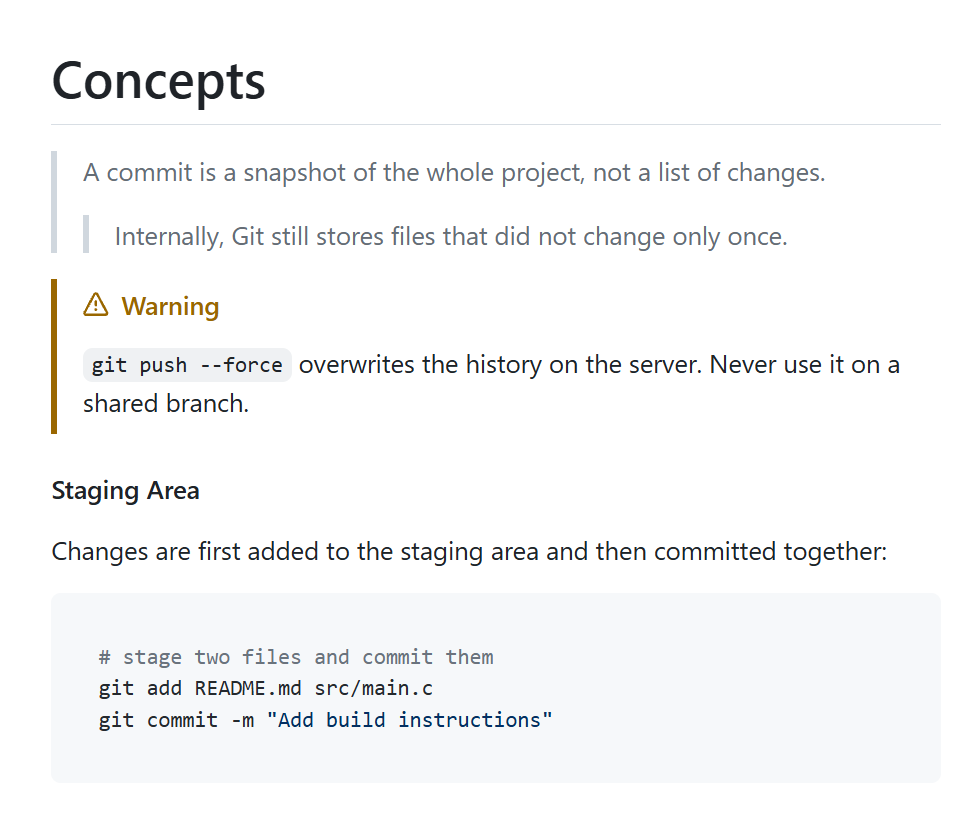
\includegraphics[height=0.45\columnwidth]{figures/screenshots/substitutes-preview}\hfill
	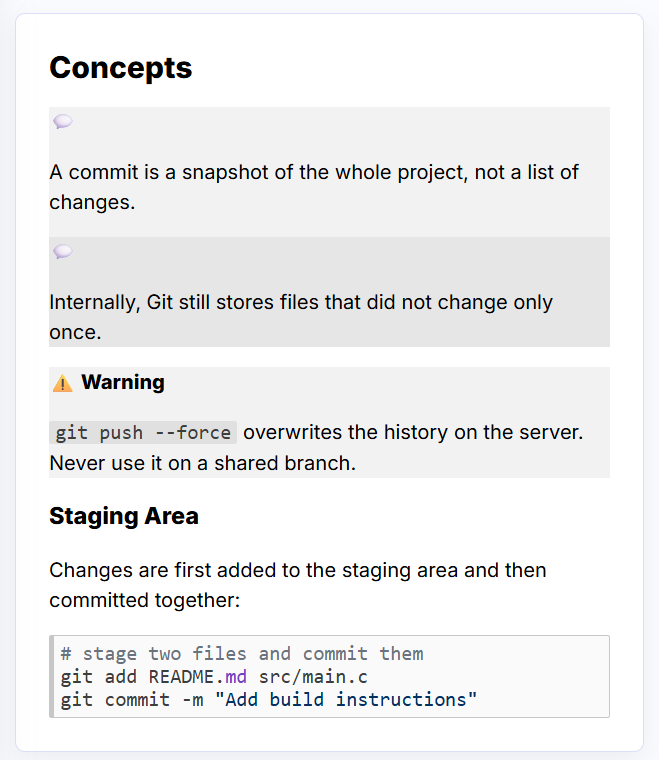
\includegraphics[height=0.45\columnwidth]{figures/screenshots/substitutes-moodle}
	\caption[Substitutes for unsupported tags next to a Markdown preview]{\label{fig:substitutes}The substitutes for unsupported tags next to the Markdown
		preview they stand in for.}
\end{figure}

\paragraph{Code Blocks.}
A fenced code block becomes \code{pre} and \code{code}, which are both permitted.
Without further styling, however, it is plain monospace text on the page background, since
\code{pre} is not styleable and no H5P stylesheet styles it.
The converter therefore wraps it in a \code{div} with a light background, as for block quotes.
The shade differs from the block quote grays, so that a code block inside a block quote remains
visible.
\autoref{fig:substitutes} shows the substitutes of this section next to the Markdown preview.

\subsection{Raw HTML}
\label{sec:mk_rawhtml}

Markdown permits raw HTML, both as a block and inline, and documentation written for the web uses
it for things Markdown lacks, such as a centered image or a collapsible section.
Mapping every HTML tag to something the platform accepts would mean guessing the author's intent,
and rejecting raw HTML would break documents that work everywhere else.
The converter therefore passes raw HTML through unchanged.
Moodle's sanitizer then removes the tags it does not allow.
Many of them are permitted anyway, such as \code{div}, \code{p}, \code{span}, \code{a}, and
\code{strong}.

The converter does emit warnings, however.
All raw HTML fragments are collected and checked at the end of the chapter
against the tag list of \autoref{tab:allowed} and for balanced tags.
The check covers the whole chapter, because a tag opened in one inline fragment and closed in
another is balanced.
Balance matters because Moodle's sanitizer is a regular-expression filter that does not repair the
markup\footnote{\raggedright \code{filter\_xss} in \code{h5p.classes.php}, lines 4912--5023, a port of
Drupal's filter of the same name.}~\cite{H5P:PhpLibrary}, so an unclosed tag remains open and can affect the rest of the
page.
The warning names the tags that will be removed and the tags that are not closed.
The converter does not repair either.

\newpage
\section{Content Blocks and Placement}
\label{sec:blocks}

The preceding rendering rules cover what can be expressed as markup inside a Text block.
This section covers what cannot.
Images and tables, which nearly every documentation chapter contains, have no tag and no substitute
in a Text block, so they have to become separate content blocks next to the text.
Placement is simple as long as an image stands between two paragraphs.
However, it becomes difficult when the image is inside a list item, a block quote, a table cell, or a
footnote, because the enclosing construct then has to be interrupted and resumed, and these
constructs can be nested.

\paragraph{One Renderer per Difficult Construct.}
The document visitor handles the simple node-to-tag mappings: text,
emphasis, headings, lists, and alerts.
Every construct that interrupts text or whose output depends on something outside the node
has its own renderer class in md2h5p's source code.
Separate renderers handle tables, images, footnotes, and links, as well as highlighted code and
questions.

\subsection{Images and Tables as Content Blocks}
\label{sec:mk_blocks}

Neither \code{img} nor \code{table} is permitted in a Text block (\autoref{tab:allowed}).
For \code{img}, there is no library that permits it in any text field.
A CSS \code{background-image} on a \code{div} does not work either, since the declaration is removed
by the sanitizer.
A relative URL inside it would not be resolved either, because the platform only rewrites the paths
of image parameters.
There is thus no way to put an image into a Text block.

\begin{figure}[H]
	\centering
	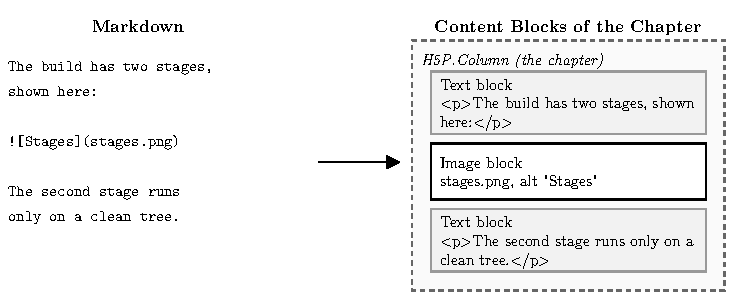
\includegraphics[width=0.9\columnwidth]{figures/block-split}
	\caption[An image splits a chapter into three blocks]{\label{fig:block_split}An image between two sentences splits the chapter into three
		content blocks: the text before it, the image, and the text after it.
		The reader sees a
		continuous page; the package holds three entries in the chapter's column.}
\end{figure}

Both constructs, however, exist as content types of their own, \code{H5P.Image} and
\code{H5P.Table}.
An image or a table therefore becomes a block after the text instead of markup inside
it.
As a consequence, a paragraph containing an image is no longer one block.
\autoref{fig:block_split} shows the simplest case: the text before the image is flushed into a Text
block, the image becomes an Image block, and the text after it starts a new Text block.
The same happens to a table in the middle of a chapter.
The reader does not notice the split, since the blocks of a column follow each other without a gap.
For an image at the top level of a chapter, this is all that is needed.

\subsection{Tables and Images}
\label{sec:mk_pseudotable}

A table without images becomes one \code{H5P.Table} block.
For example, the two-column Markdown table in \autoref{fig:regular_table} becomes a table with a
header row and two data rows.
Its HTML uses \code{table}, \code{thead}, \code{tbody}, \code{tr}, \code{th}, and \code{td}, which
are permitted in a Table block (\autoref{tab:allowed}).
The cells are also styled with borders, padding, and alignment.
The whole table remains editable as one table in the H5P editor.

\begin{figure}[H]
    \centering
    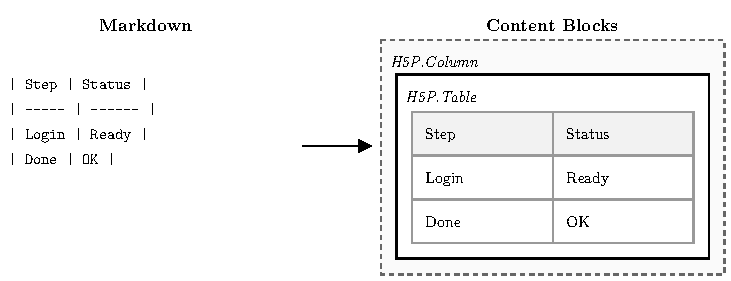
\includegraphics[width=\columnwidth]{figures/regular-table}
    \caption[A regular table as one content block]{\label{fig:regular_table}A Markdown table without images (left)
        becomes one \code{H5P.Table} block in the chapter's \code{H5P.Column} (right).}
\end{figure}

\paragraph{Images Inside Cells.}

In Markdown, a table cell may contain an image, but in a Table block it may not. A table cannot be
split around the image the way a list or a quote can.
Instead, the converter builds such a table from layout blocks.
The layout library \code{H5P.Row} places its \code{H5P.RowColumn} children side by side, and each of
them holds a vertical list of blocks, which may include Table blocks and Image blocks.
A table with an image is therefore rebuilt as one Row per table row and one RowColumn per cell.
Each cell is a vertical stack of its text as a one-cell Table block, its image as an Image block, and
any further text as another Table block.
\autoref{fig:pseudo_table} shows the structure for a two-by-two table.
The image-containing cell illustrates the split into a Table block, an Image block, and another Table block.
The result is called a \emph{pseudo-table}.

\begin{figure}[H]
	\centering
	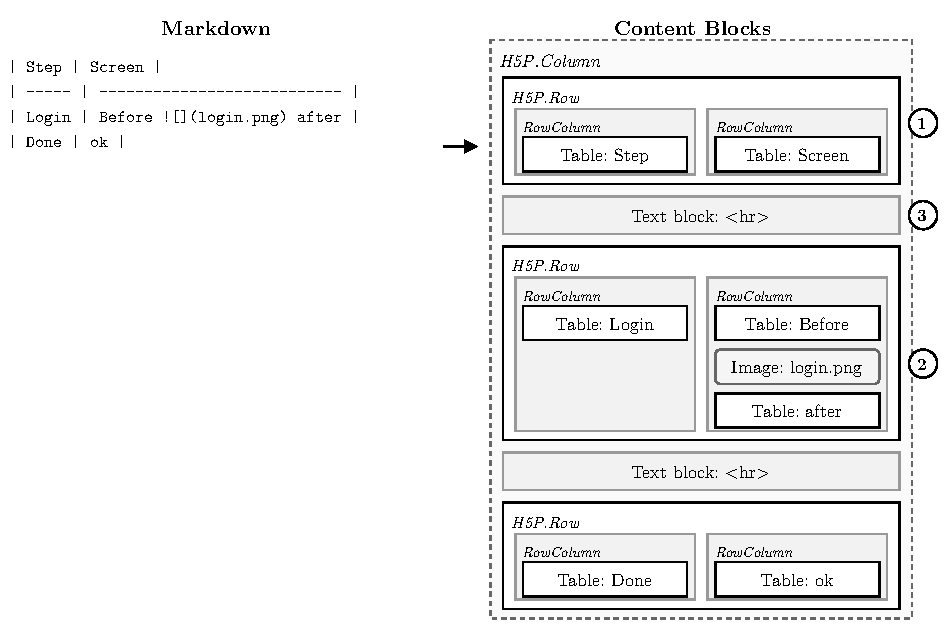
\includegraphics[width=\columnwidth]{figures/pseudo-table}
	\caption[A table with an image rebuilt as a pseudo-table]{\label{fig:pseudo_table}A Markdown table with an image, rebuilt from the layout
		library.
		Every table row becomes an \code{H5P.Row} \circled{1}, every cell an
		\code{H5P.RowColumn} holding a vertical stack of one-cell Table blocks and Image blocks
		\circled{2}, and the row boundary is a horizontal rule \circled{3} in a Text block of its own,
		drawn across the full width.}
\end{figure}

The cell's text is represented by a one-cell Table block instead of a Text block, because \code{padding} is
only available for libraries that permit \code{table} (\autoref{tab:allowed}).

The pseudo-table looks different from regular tables because its cells have no borders.
Borders around the one-cell Table blocks would frame individual text fragments rather than the
whole Markdown cell: an image can split one cell into several such blocks.
Instead, a shaded header row and full-width horizontal rules give the pseudo-table its structure.
Each rule is a separate Text block containing only \code{hr}, placed between adjacent rows.

\paragraph{Four-Column Limit.}
The pseudo-table solution works only for tables with \emph{at most four columns}, the maximum
\code{H5P.Row} permits in its \code{semantics.json}.
From five columns onward, the converter must use a regular Table block and a different fallback:
the image's alternative text becomes a placeholder in the cell, and the image itself is placed
immediately after the table.
A warning reports this displacement.
The table keeps its grid, but the image loses its position inside the cell.
\autoref{fig:pseudo_table_shot} contrasts the pseudo-table with this fallback.

\begin{figure}[H]
	\centering
	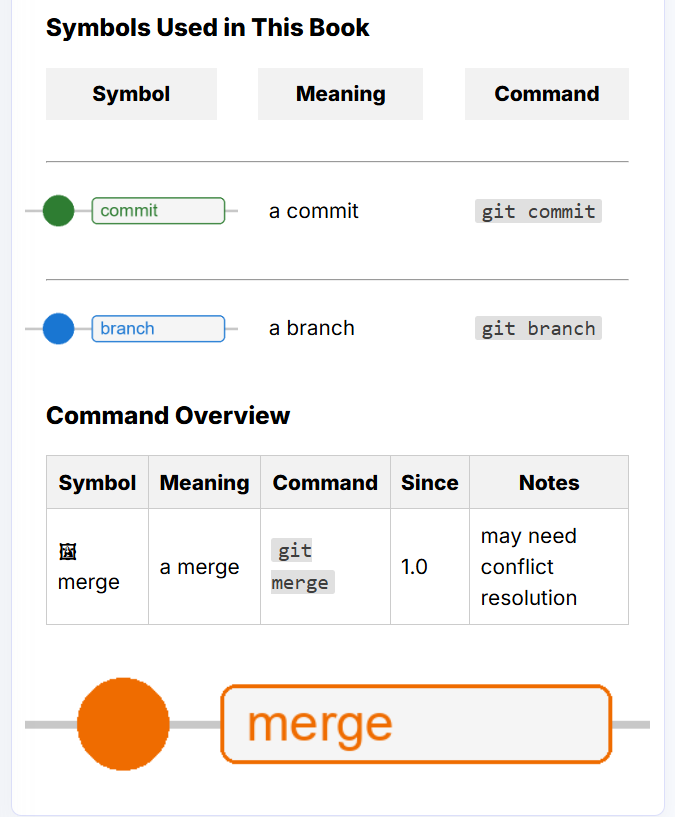
\includegraphics[width=0.75\columnwidth]{figures/screenshots/pseudo-table}
	\caption[A pseudo-table and a real table with the image lifted out]{\label{fig:pseudo_table_shot}A table with an image as a pseudo-table (top) and, above
		four columns, as a real table with the image lifted out (bottom).}
\end{figure}

The pseudo-table has several drawbacks.
In the H5P editor, it is no longer an editable table but a tree of rows and columns.
It also looks different from the other tables of the book.
Below a viewport width of 480 pixels, the layout library stacks its columns vertically, so on a phone
the table becomes a list.
Finally, it requires two additional libraries in the package.
The pseudo-table is therefore only used for tables that contain an image.

The regular table and the pseudo-table need different ways to receive an image.
This placement depends on the enclosing construct, a problem that also occurs in lists and block quotes.

\subsection{Placement Through Render Contexts}
\label{sec:bl_context}

An image needs different placement depending on what encloses it.
At chapter level, it interrupts the text; inside a pseudo-table cell, it joins the cell's vertical
stack of blocks.
Lists, block quotes, and footnotes also need to make room for images.
If the image renderer handled every enclosing construct itself, each new construct would add
another case to that renderer.

The renderer therefore keeps a stack of \emph{render contexts}.
Each context decides how to place a content block, such as a table or an image, inside its enclosing construct.
The page context is always present; rendering a pseudo-table cell pushes a cell context onto the stack.
The image renderer can then build a block independently and hand it to the innermost context for placement.

\begin{figure}[H]
    \centering
    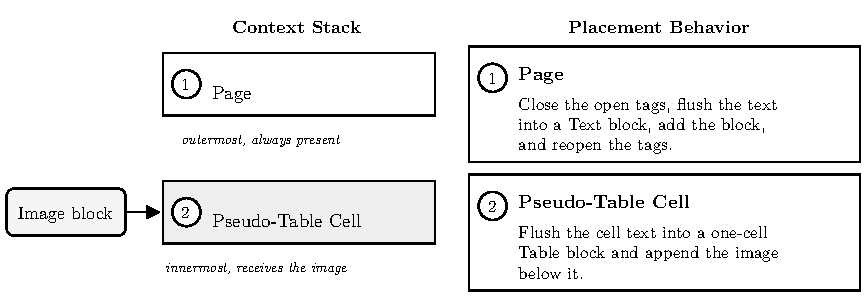
\includegraphics[width=\columnwidth]{figures/render-contexts}
    \caption[Placement of an image inside a pseudo-table cell]{\label{fig:render_contexts}The contexts
        for an image inside a pseudo-table cell, from the outermost context at the top to the
        innermost below. Each context on the left has its placement behavior shown opposite it.
        The image is handed to the cell context \circled{2}.}
\end{figure}

\autoref{fig:render_contexts} contrasts the two placement behaviors.
The page context \circled{1} closes the open tags, flushes the text into a Text block, adds the
new block to the chapter, and reopens the tags.
This produces the split shown in \autoref{fig:block_split}.
The pseudo-table cell context \circled{2} instead flushes its text into a one-cell Table block
and appends the image below it in the same column.
Further text becomes another one-cell Table block, producing the Table--Image--Table sequence
of \autoref{fig:pseudo_table}.
After the cell has been rendered, its context is removed and the previous context becomes active again.

The image renderer therefore needs no knowledge of tables.
The same mechanism also handles a table inside a block quote: the page context closes the
shaded box and reopens it after the table.
When questions were added, they were placed like any other
block, and none of the contexts had to be changed.

The page context also keeps the state of numbered lists.
Reopening an \code{ol} creates a new list, which HTML numbers from one by default.
If the third item contains an image, the fourth item would start at 1 again without an explicit start number, yielding 1, 2, 3, 1.
The page context therefore records where a list began and gives the reopened list an explicit
\code{start}.

Footnotes likewise use a separate context to interrupt and resume their numbered list.

\subsection{Footnotes}
\label{sec:bl_footnotes}

A Markdown footnote consists of a reference such as \code{[\textasciicircum{}term]} in the text
and a matching definition introduced by \code{[\textasciicircum{}term]:}.
A renderer replaces the reference with a number and displays the explanation at the end of the document.
\autoref{fig:footnotes} shows a basic example and its conversion to H5P.

\begin{figure}[H]
    \centering
    \begin{minipage}[t]{0.34\columnwidth}
        \centering
        \textbf{Markdown Source}\par\smallskip
\begin{lstlisting}[basicstyle=\ttfamily\scriptsize,frame=none,xleftmargin=0pt,framexleftmargin=0pt]
A short note explains
the term.[^term]

[^term]: This is the explanation.
\end{lstlisting}
    \end{minipage}\hfill
    \begin{minipage}[t]{0.31\columnwidth}
        \centering
        \textbf{Markdown Preview}\par\smallskip
        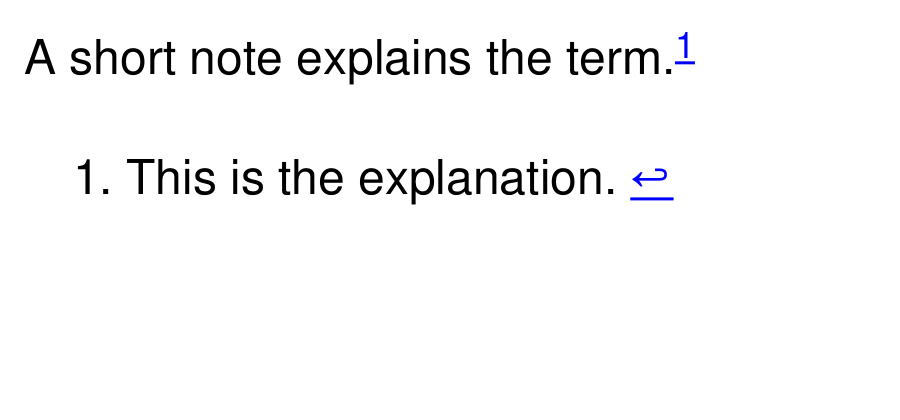
\includegraphics[width=\linewidth]{figures/screenshots/footnotes-preview}
    \end{minipage}\hfill
    \begin{minipage}[t]{0.31\columnwidth}
        \centering
        \textbf{Moodle}\par\smallskip
        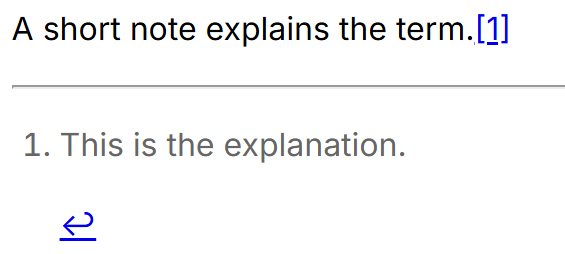
\includegraphics[width=\linewidth]{figures/screenshots/footnotes-moodle}
    \end{minipage}
    \caption[Footnotes in Markdown and Moodle]{\label{fig:footnotes}A footnote in Markdown source (left),
        in a commonmark-java HTML preview (middle), and after conversion in Moodle (right).}
\end{figure}

The converter represents the footnotes as an ordered list at the end of the chapter, separated
from the text by a horizontal rule.
References appear as bracketed numbers such as \code{[1]}, since \code{sup} is not permitted
(\autoref{tab:allowed}).
Each reference links to its list entry; a back-link returns to the reference.
An image or a table inside a footnote is placed through the same render-context mechanism.

\subsection{Links}
\label{sec:rf_anchors}

The output for a link cannot be determined from its node alone.
A Markdown link has a destination, and what the converter emits depends on where that destination
points, which in turn depends on the whole book.

\paragraph{Four Kinds of Link.}
A destination falls into one of four classes.
\circled{1} A link \emph{within the chapter}, such as \code{[the summary](\#summary)} or the wiki
link \code{[[\#Summary]]}, is emitted as an ordinary anchor.
\circled{2} A link \emph{to another chapter}, such as \code{[Setup](2\_setup.md)} with or without a
fragment like \code{\#install}, or \code{[[Setup]]}, cannot be emitted as a working link, for the
reason given at the end of this section.
\circled{3} A link \emph{to a Markdown file that is not a chapter}, such as
\code{[notes](appendix.md)}, has no target in the book, so it becomes plain text and a warning names
the file.
\circled{4} A link \emph{out of the package}, such as \code{[H5P](https://h5p.org)}, is emitted as
it is.
Whether \code{2\_setup.md} is a chapter and what title and identifier it has is unknown until
every file has been parsed.
This is why the conversion pipeline has two passes.
Wiki links are resolved as in Obsidian, by name rather than by path: an author writes
\code{[[Setup]]} instead of \code{[[2\_Setup.md]]}.
A chapter can therefore be referenced by its file name, by the file name without its number prefix,
and by its title.

\paragraph{Anchors per Chapter.}
Every heading gets an \code{id} derived from its text, so that links within the chapter can refer
to it.
Similarly, \code{id} attributes are attached to the footnote references and back-links.
However, an Interactive Book keeps several chapters in one HTML document, so ids must be unique across chapters.
Otherwise, links jump to the first element with the matching id.
To prevent a heading such as ``Summary'' from producing two elements with the same id across chapters,
the converter prefixes every id a chapter generates with \code{ch<n>-} and rewrites every
in-page link accordingly.
For example, \code{[x](\#summary)} in chapter~3 becomes \code{href="\#ch3-summary"}.
This works because the converter generates both the ids and the links.
An id written by hand in raw HTML, however, is not rewritten, since raw HTML is passed through unchanged; a Markdown link to such an anchor therefore does not work.

\paragraph{Links Between Chapters.}
\label{sec:rf_crosschapter}
The converter cannot generate working links between chapters because of how Interactive Book navigates.
It uses a URL fragment of the form
\code{\#h5pbookid=<id>}\allowbreak\code{\&chapter=<chapter-id>}\allowbreak\code{\&section=<element-id>}.
The player compares \code{h5pbookid} with the content id of the running book before it
navigates~\cite{H5P:InteractiveBook}.
The other parts of the fragment, however, are known at conversion time.
The chapter id is derived from an identifier the converter writes into the package, and the section
is the anchor's id.
The missing value is the content id, which Moodle assigns when the content is first viewed.
A package cannot choose this value, and Moodle assigns a new one when a changed package is uploaded~\cite{Moodle:Source}.
A custom library that navigates in JavaScript, as the sidebar does, would have to be added to the
content types the column accepts, which would require a modified copy of the column library.

\begin{figure}[H]
	\centering
	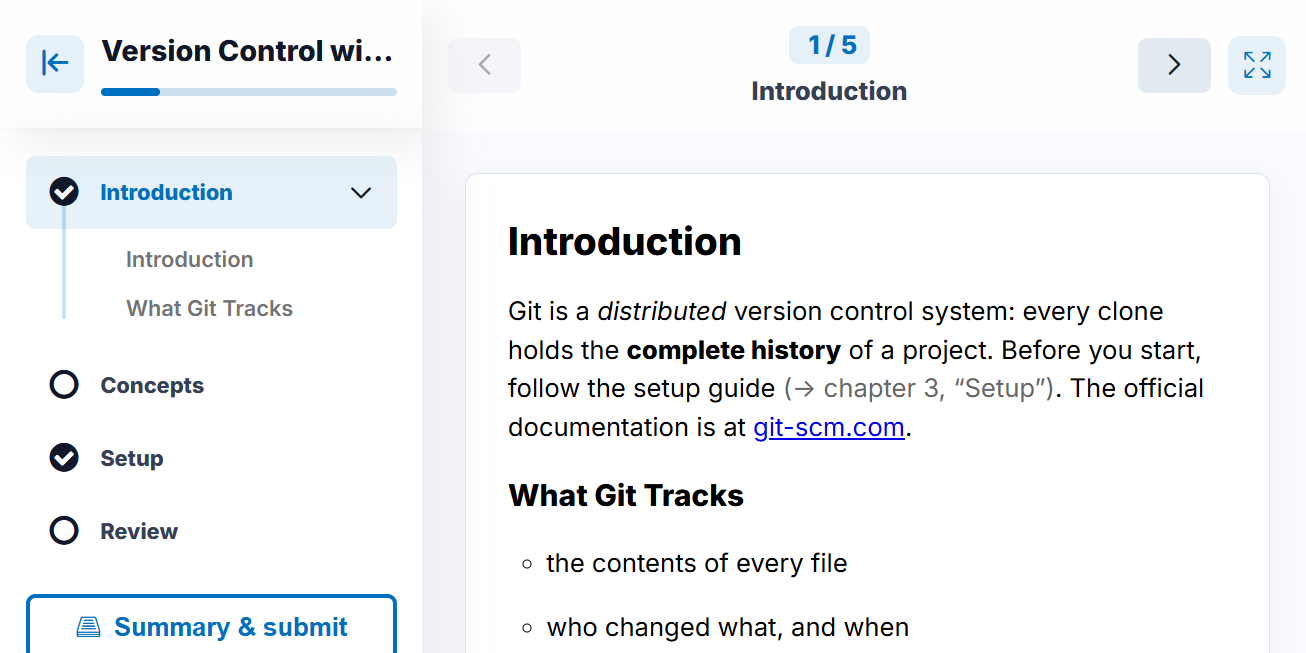
\includegraphics[width=\columnwidth]{figures/screenshots/crosschapter}
	\caption[A reference to another chapter]{\label{fig:crosschapter}A reference to another chapter as the converter renders it,
		next to the sidebar entry it points the reader to.}
\end{figure}

Instead, the converter keeps the link text and appends a muted, non-clickable note with the number
and title of the target chapter, such as ``the setup guide (\textrightarrow{} chapter 3,
``Setup'')'', and issues a warning (\autoref{fig:crosschapter}).
Since every heading is listed in the book's sidebar, which is open by default, the reader can reach
the target with two clicks.

\newpage
\section{Syntax Highlighting, Formulas, and Questions}
\label{sec:extensions}

The previous sections covered standard Markdown and the constructs the common dialects agree on.
Lecture notes often contain three more things.
Code blocks are standard, but many Markdown viewers color them while the platform does not.
Formulas are usually written with dollar signs, but the platform only renders them in a different
notation.
Single- and multiple-choice questions, supported by H5P, have no syntax in Markdown at all.
To bridge these differences, the converter colors code during conversion and translates formula delimiters.
It also adds a syntax for questions that remains valid Markdown in other tools.

\subsection{Syntax Highlighting}
\label{sec:ex_code}

Markdown renderers commonly use a fenced code block's info string (the text after the opening backticks) to identify its language and apply appropriate syntax highlighting.
Neither Moodle nor the H5P libraries include a highlighter, and a package cannot bring one, since
\code{script} is removed by the sanitizer and JavaScript files cannot be included as content assets.
The coloring therefore has to happen during the conversion, and the colors have to be part of the
markup, i.e., applied via a tag.
The tag has to be permitted, styleable via the \code{color} property, and suitable for representing inline content,
making \code{span} the best fit (\autoref{tab:allowed}).

The converter splits every fenced code block into tokens and wraps every colored token in
\code{<span style="color:\#\ldots">}.
For this tokenization, the converter uses the lexer of RSyntaxTextArea~\cite{RSyntaxTextArea}, a Java
text component whose highlighting engine can be used without its graphical parts.
It supports more than 50 languages and 39 token types and keeps the state of multi-line comments across lines.
The converter maps the first word of a fence's info string to one of these languages, and each token
type to a color chosen for the light background of the code box.
To limit the size of the generated JSON, adjacent tokens with the same color are merged into one
span.
Identifiers, whitespace, separators, and operators, which make up the bulk of a file, receive
no span at all.
For a language without a mapping, the block remains uncolored, and one warning is issued per language
and chapter.
Some mappings are approximations: TOML is tokenized as INI and \code{.env} files as Java properties.

Three alternatives were considered.
Prism4j, a Java port of the Prism.js highlighter, supports about twenty languages but has not been
maintained since 2019.
highlight.js on the GraalVM JavaScript engine supports far more languages but requires a JavaScript
runtime in the distribution.
A custom lexer would have no dependency but would have to be written for every language.
Even so, the chosen approach has two drawbacks.
The generated \code{content.json} grows, since a colored block is several times the size of a plain
one.
The colors are also fixed, so they do not adapt to a dark mode or to the Moodle theme, since no
stylesheet can be shipped.

\subsection{Formulas}
\label{sec:ex_math}

Most Markdown editors and viewers render \code{\$x\$} as an inline formula and \code{\$\$x\$\$} as a
displayed one.
In H5P, formulas are rendered by \code{H5P.MathDisplay}, a site-wide add-on that an administrator
installs and that renders formulas in any content whose text matches its delimiters.
It recognizes \code{\textbackslash(x\textbackslash)}, \code{\textbackslash[x\textbackslash]}, and
\code{\$\$x\$\$}, but not a single dollar sign, and the delimiters cannot be configured in current
versions~\cite{H5P:MathDisplay}.
Only \code{\$\$x\$\$} is therefore understood by both sides, but the most common Markdown notation for
inline formulas would be displayed as literal dollar signs.

The converter recognizes both dollar notations and only rewrites the one that needs it.
\code{\$x\$} becomes \code{\textbackslash(x\textbackslash)}, while \code{\$\$x\$\$} is kept as it is,
so that it also reads correctly on a site without the add-on.
On the H5P side, nothing else is needed, since the add-on finds the delimiters in the rendered page.
On the Markdown side, a custom extension to commonmark was implemented.
Without it, commonmark would interpret the asterisks in \code{\$a*b*c\$} as emphasis.
The extension changes single-dollar delimiters to \code{\textbackslash(} and \code{\textbackslash)} and prevents the formula's contents from being interpreted as Markdown.
Since \code{\$5} and \code{\$PATH} are common in documentation, though, single-dollar formulas need a rule.
The converter uses that of Pandoc: no whitespace directly inside either delimiter and no digit right
after the closing one.
As a consequence, \code{\$ x \$} is not recognized as a formula.

The backslash notations are not treated as formulas in the source.
Markdown editors generally do not render \code{\textbackslash(x\textbackslash)} as math, so an author who wrote it
meant an escaped parenthesis, and their preview shows \code{(x)}.
commonmark's backslash escape already turns \code{\textbackslash(} into \code{(}, so the add-on finds
no delimiter.
Even with these delimiter changes, two limitations remain.
Formulas are only rendered if the add-on is installed, which the package cannot check; otherwise the
reader sees \code{\textbackslash(E = mc\textasciicircum{}2\textbackslash)}.
Furthermore, a vertical bar inside a formula still splits a table cell, since the table extension
determines the cell boundaries before inline parsing.

\subsection{Interactive Questions}
\label{sec:ex_quiz}

Markdown has no syntax for questions, so one has to be defined.
The main requirement is that the file still works in every other tool the author uses, such
as Obsidian, GitHub's viewer, or an editor's preview.
A format that only this converter can read would no longer be Markdown.
The syntax therefore has to render as something sensible in other tools, and its content has to be
protected from other parsers, since it is not prose.

A fenced code block meets both requirements.
It is part of CommonMark and thus supported by every tool, its content is taken literally, and its
info string is free text without a predefined meaning.
In other tools, the author sees a small monospaced box with the question and its answers.
\autoref{lst:quiz} shows the syntax.
The info string names the question type (\code{singlechoice} to create an \code{H5P.SingleChoiceSet} block and \code{multiplechoice} for an \code{H5P.MultiChoice} block), the first line is the question, and every further line is an
answer.
A leading asterisk marks a correct answer.

\par\medskip
\noindent\begin{minipage}{\linewidth}
\begin{lstlisting}[morecomment={[l][\color{blue!60!black}]{```}},caption={[Example questions as fenced code blocks]A single-choice and a multiple-choice question as fenced code blocks.
The info string selects the type, the first line is the question, and a leading asterisk marks a
correct answer.},label={lst:quiz}]
```singlechoice
What is the capital of Austria?
Salzburg
*Vienna
Linz
```

```multiplechoice
Which of these are H5P content types?
*Interactive Book
Markdown
*Course Presentation
\*.h5p (this answer starts with a literal asterisk)
```
\end{lstlisting}
\end{minipage}

The info string could also support future extensions, such as flashcards and fill-in-the-blank questions.

\begin{figure}[H]
	\centering
	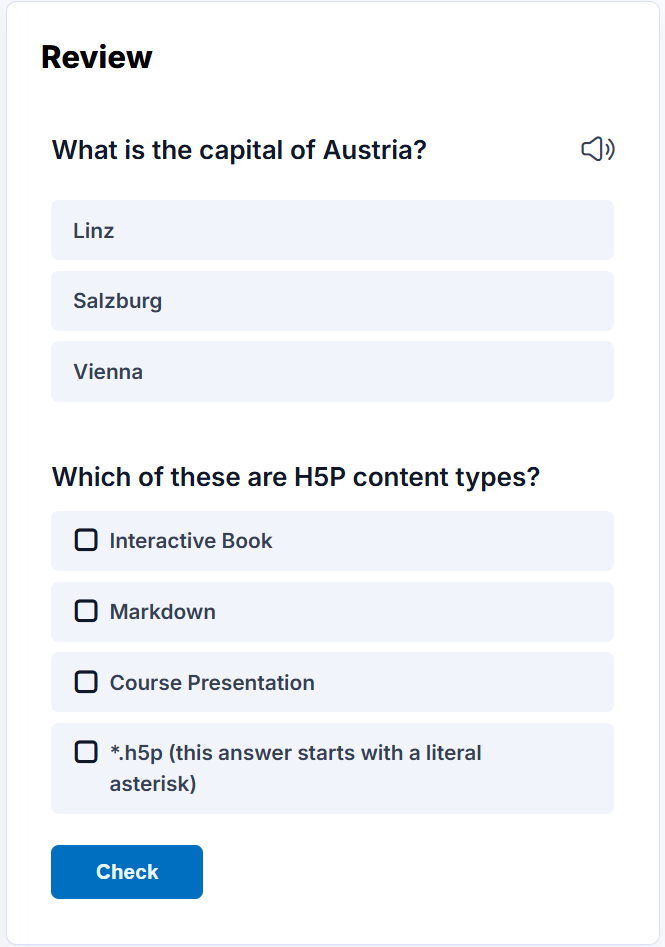
\includegraphics[width=0.55\columnwidth]{figures/screenshots/quiz}
	\caption[The example questions in Moodle]{\label{fig:quiz}The questions of \autoref{lst:quiz} in Moodle.}
\end{figure}

\autoref{fig:quiz} shows both questions of \autoref{lst:quiz} as the reader sees them.

A block that cannot become a question because it is empty, has no answers, only one answer, or
no correct answer becomes an ordinary code block with a warning naming the problem.

\newpage
\section{Merging Edited Packages}
\label{sec:merge}

\begin{figure}[H]
	\centering
	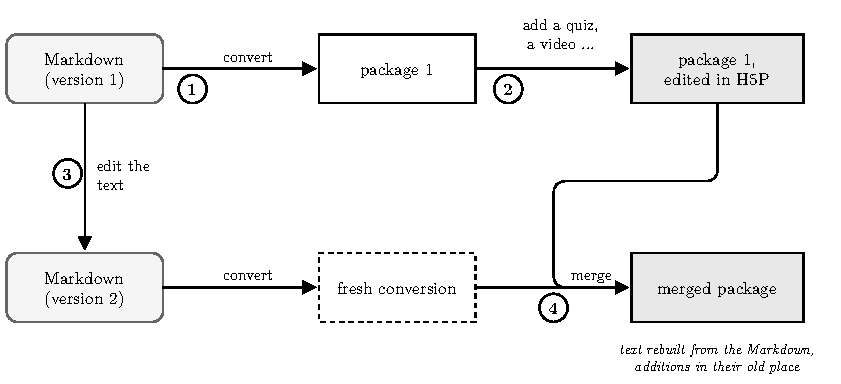
\includegraphics[width=0.95\columnwidth]{figures/merge-workflow}
	\caption[The editing cycle the merge exists for]{\label{fig:merge_workflow}The editing cycle the merge exists for.
	The Markdown is
		converted \circled{1}, the package is extended in the H5P editor \circled{2}, the Markdown
		changes \circled{3}, and the fresh conversion is merged with the edited package \circled{4}:
		the text is rebuilt from the Markdown, the additions keep their place.}
\end{figure}

The previous sections described a one-way conversion.
In practice, a teacher converts their notes, uploads the book, and then adds content in the H5P
editor that Markdown cannot express, such as a video, an image with hotspots, or a question type
that the question extension does not cover.
When the notes change later, a new conversion produces a package without these additions, and the
teacher would have to transfer them by hand.
\autoref{fig:merge_workflow} shows this cycle.
The converter therefore accepts the edited package as a second input \circled{4} to merge it with
the new conversion.

\subsection{Merge Policy}
\label{sec:mg_policy}

A three-way merge would have to reconcile the original Markdown, the revised Markdown, and the
edited H5P package.
If the same text is changed in both Markdown and H5P, the edits can conflict and require manual
resolution, as in a Git merge.
The converter avoids this complexity by preserving only additions from the H5P editor and dropping any edits to generated blocks, though warnings are issued for them.
The new Markdown conversion therefore replaces all generated blocks.
The remaining task is to place the manually added blocks among the newly generated blocks.

\subsection{Block Markers}
\label{sec:mg_markers}

For every block of the edited package, the merge has to know whether it came from Markdown or was manually added.
The package must therefore record the origin of its blocks in a form that survives an upload,
an editing session, and an export.

\begin{figure}[H]
	\centering
	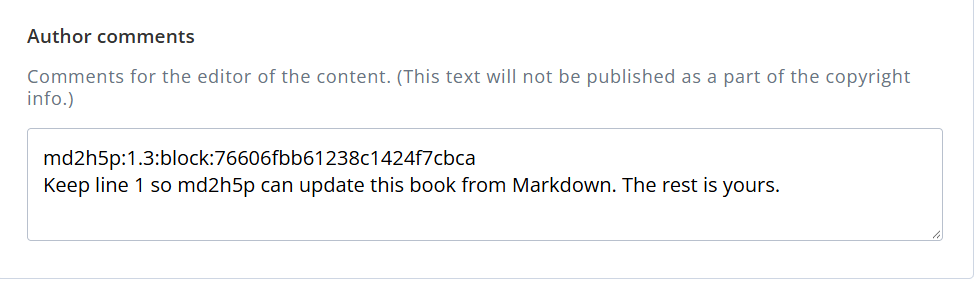
\includegraphics[width=0.9\columnwidth]{figures/screenshots/marker-comments}
	\caption[A marker in the metadata dialog of the H5P editor]{\label{fig:marker_dialog}The Author comments field
		of a generated block in the H5P editor's metadata dialog.}
\end{figure}

The converter records a marker in each generated chapter and top-level block, using the
\code{metadata.authorComments} field shown in \autoref{lst:marker}.
The first line contains a fixed prefix, the converter's version, the kind of element, and for a block
a hash of its content or for a chapter the name of its Markdown file.
The second line explains the purpose of the first one, since the field is visible to the teacher in
the metadata dialog of a block (\autoref{fig:marker_dialog}).

\par\medskip
\noindent\begin{minipage}{\linewidth}
\begin{lstlisting}[caption={[A block marker in \code{content.json}]A marker as it sits in \code{content.json}: the \code{authorComments}
field of one Text block, with the machine-readable first line and the explanation on the second.},
label={lst:marker}]
{
  "library": "H5P.AdvancedText 1.1",
  "params": { "text": "<p>The build has two stages, ...</p>" },
  "metadata": {
    "title": "Untitled Text",
    "authorComments": "md2h5p:1.3:block:18be0e19a4ab2eba443b37a2\nKeep line 1 so md2h5p can update this book from Markdown. The rest is yours."
  },
  "subContentId": "454e712b-26bd-aa20-f872-0941fa480cd8"
}
\end{lstlisting}
\end{minipage}

A marker alone suffices for identifying a block as generated from Markdown.
Unmarked blocks are consequently treated as manually added, even if their marker was deleted in the editor.
The marker's hash also detects changes to the block's content while ignoring metadata, whitespace
differences, and HTML tags to avoid reporting automatic editor changes.
Though changes to generated blocks can be detected and warned about through the hash, they cannot be reconciled under the chosen merge policy and are discarded.

\subsection{Alignment and Placement}
\label{sec:mg_alignment}

The additions must now be placed among the blocks of the new conversion.
An addition may have followed a paragraph that has since been reworded, split by an image, or deleted.
The merge therefore needs to recognize the corresponding block after its Markdown has changed.
Hashes alone cannot do this: even a typo correction changes the hash.

\paragraph{Block Similarity.}
An addition is anchored to the nearest preceding Markdown-generated block.
Consecutive additions are kept together in their original order.
Even if the anchor block has been reworded, it still likely resembles a block in the new conversion.
To find the counterpart and place the additions after it, the merge needs a measure of similarity.

The S{\o}rensen--Dice coefficient~\cite{Dice:1945} measures the overlap between two multisets.
Here, it is applied to adjacent word pairs extracted from the blocks' text.
Using word pairs rather than individual words makes the comparison stricter, since the words must
also occur next to each other in the same order to count toward similarity.
The coefficient divides twice the number of shared pair occurrences by the total number of pairs
in both texts.
Let $A$ and $B$ be the multisets of adjacent word pairs from two texts.
Their similarity is
\begin{equation}
    D(A,B) = \frac{2|A\cap B|}{|A|+|B|}.
    \label{eq:merge_dice}
\end{equation}
Here, $|A|$ and $|B|$ count word-pair occurrences; the intersection counts shared occurrences, including repetitions.
The result lies between 0 and 1, giving comparisons of different blocks a common scale.
A score of 0 means no shared pairs; 1 means identical pair counts, which does not necessarily imply
identical text.
\autoref{fig:merge_dice} gives a small example.

\begin{figure}[H]
    \centering
    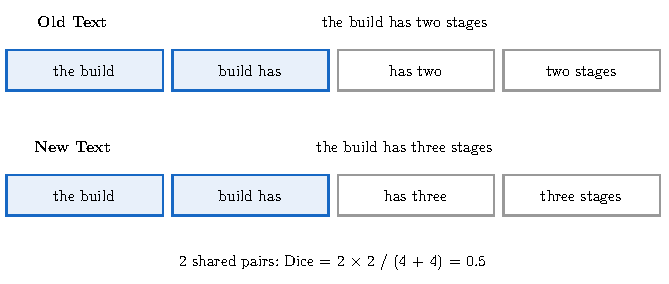
\includegraphics[width=\columnwidth]{figures/merge-dice}
    \caption[Similarity from adjacent word pairs]{\label{fig:merge_dice}Each text has four adjacent
        word pairs. Two pairs are shared (shaded), giving a similarity of $2\cdot2/(4+4)=0.5$.}
\end{figure}

Counting the word pairs in a hash table gives an expected running time of $O(m+n)$ for texts of
lengths $m$ and $n$.
This keeps each comparison inexpensive, which matters because every old block is compared with every new block.
Edit-distance measures are another option, but were not chosen because a standard Levenshtein
computation takes $O(mn)$ time for each comparison.

The text is taken only from the block's actual text, after removing all tags and metadata.
To prevent mix-ups between different kinds of blocks, two blocks of different libraries score 0.0, since a table or a question
never corresponds to a text block.

\paragraph{Alignment.}
Knowing how similar blocks are is not enough to place the additions.
Repeated passages may match several candidates, and a single old block may have been split into
several new ones.
The merge therefore needs a separate alignment algorithm to establish which blocks correspond.
The old and the new blocks of a chapter are aligned with the Needleman--Wunsch
algorithm~\cite{Needleman:1970}, a standard method for sequence alignment.
It considers block pairs with a S{\o}rensen--Dice score of at least 0.35 and finds the pairing with
the highest total score in which no two pairs cross.
This preserves the order of the blocks in the chapter.

\begin{figure}[H]
	\centering
	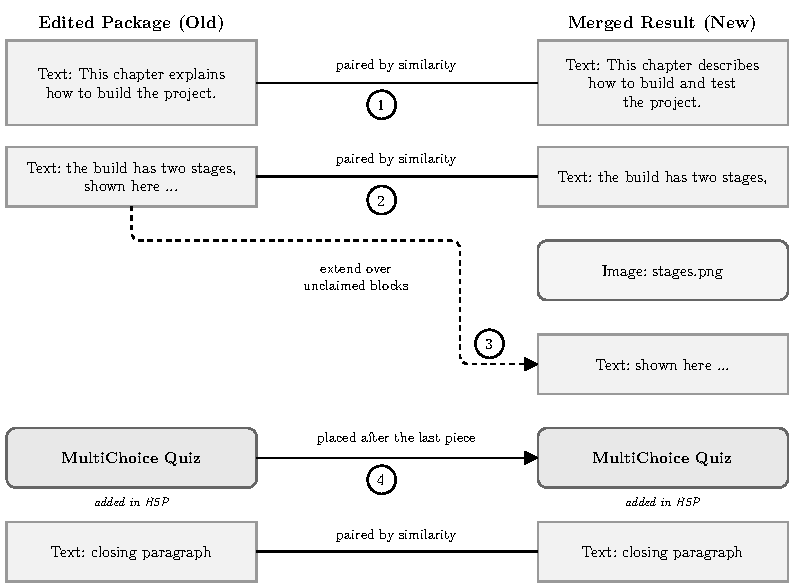
\includegraphics[width=\columnwidth]{figures/merge-alignment}
	\caption[Aligning the blocks of an edited chapter with the fresh conversion]{\label{fig:merge_alignment}Aligning the blocks of an edited chapter with the fresh
		conversion.
		Reworded blocks are paired by similarity \circled{1}~\circled{2}.
		A paragraph split by a new image is one old block and a run of new ones, so
		the anchor walks forward over the blocks nothing else claimed \circled{3}, and the quiz is
		placed after the last piece of the run \circled{4}.}
\end{figure}

\autoref{fig:merge_alignment} shows a chapter in which the introduction was reworded \circled{1}, a
paragraph was split by a new image \circled{2}, and a quiz had been added after that paragraph.
An addition remembers the block it followed and is placed after the block that one became
\circled{4}.

The split requires an additional step \circled{3}.
When an image is inserted into a run of paragraphs, the renderer emits text, image, and text where
there was a single Text block before.
One old block thus corresponds to a run of new blocks, and an addition that followed it
belongs after the last of them.
After the alignment, the merge scans the following unpaired blocks up to the first block paired
with another old block.
The anchor moves to the last of these blocks with a similarity of at least 0.15 to the old block.
Blocks in between, such as the new image, need not resemble it.
Conversely, if an image is removed, multiple blocks may become a single Text block.
The alignment in that case pairs one of the old text blocks with this combined block; the other old blocks
remain unpaired.

Two structural rules take precedence over the scores.
An addition at the very beginning stays first, and an addition that followed
the last block stays last, regardless of what the Markdown appends.
Only for a block that no longer exists does the merge have to guess.
It uses the nearest earlier block that still exists, then the nearest later one, and finally the end
or the beginning of the chapter, depending on which one is closer.
Only this case produces a warning.

This order-preserving alignment cannot represent a reordering.
If two paragraphs swap places in the Markdown, both cannot be paired correctly without crossings,
so a quiz added after one of them may end up after the wrong paragraph.
The text itself is not affected, since it is regenerated; only the additions may be misplaced.
The merge detects this case: if an old block scored strictly higher against a block it was not paired with, and the chapter
contains additions, the merge warns that the chapter appears to have been reordered.

\subsection{Chapters and Package Assembly}
\label{sec:mg_result}

\paragraph{Chapter Alignment.}
Changes to the Markdown source can also affect the naming or ordering of chapters.
To account for that, chapters are aligned in the same way, with a score determined in four steps.
Two chapters with the same source file name are the same chapter.
Otherwise, chapters with the same title are the same chapter.
Otherwise, the file names are compared after removing the number prefix and the extension and
normalizing punctuation, so that \code{3\_Retired.md} and
\code{03 - Retired.md} have the same name.
This step allows a book to be renumbered, which happens whenever a chapter is inserted in the middle.
Otherwise, the text of the chapters is compared like that of blocks.
This allows the merge to recognize the same chapter even if both its file name and its first heading
have changed.
A similar file name only adds a small bonus to the text score.
\code{3\_Basics.md} and \code{4\_Basics2.md}, for example, have very similar names but are two
different chapters.

\paragraph{Library Versions.}
A package names each library in three places that must agree: in the folder that contains it, in
the dependency list in \code{h5p.json}, and in the \code{library} field of every block.
A merge can bring them out of agreement because platforms upgrade their installed libraries, and a
package that was edited there may use newer versions.
For example, a generated book may use \code{H5P.Column 1.18}, while the edited package is automatically updated to use
\code{H5P.Column 1.22}.
Since mixing versions is not allowed by Moodle, the merged package needs to be updated to the versions of the edited package.
To do so, the merge keeps one version per library and rewrites every \code{library} field of the content accordingly.
However, the merge cannot run the migration scripts a library provides for a version change, so every version
change is reported in a warning.

\paragraph{Assembly.}
The result is built on the edited package rather than on the converter's template, so that the libraries
needed by the additions are included, even those the template does not contain.
The dependency lists of both packages are combined.
The media files must also be merged, so that media added both by the Markdown changes and
by the H5P changes sit alongside the existing ones.

With the merge, a book can be converted, extended in H5P, and converted again without losing these
additions.

\newpage

% --- closing ---
\section{Evaluation}
\label{sec:evaluation}

The previous sections discussed each decision on its own.
This section evaluates the converter as a whole: whether it works on a real book, how much of
Markdown survives the conversion and in which form, and how long a conversion takes.
\subsection{Converting a Set of Lecture Notes}
\label{sec:ev_case_notes}

The case study uses web development lecture notes provided by Prof.\ Weninger.
The corpus consists of 12 Markdown chapters; other files in the supplied folder were ignored.
Together, they contain 345,154 bytes, 339 fenced code blocks with 3,937 lines of code, 13 tables,
and 15 links.
The files cover HTML, CSS, JavaScript, Vue.js, backend development, databases, and WebSockets.
The source files were converted without corrections.

The conversion completed and produced a package of approximately 1.57 MB.
\autoref{tab:webdev_warnings} groups its four warnings.
Four HTTP examples and 35 Vue examples are displayed without syntax highlighting.
The converter reports an unknown language once per chapter, so these 39 blocks produce only three
warnings.
The remaining warning concerns an unfenced \code{<input>} tag in the advanced Vue chapter.
This tag cannot be retained in an H5P text field and is removed by the platform.
Writing it as inline code instead would preserve it as part of the explanation.

\begin{table}[htbp]
\centering
\small
\begin{tabular}{@{}>{\raggedright\arraybackslash}p{0.34\columnwidth}r>{\raggedright\arraybackslash}p{0.54\columnwidth}@{}}
\toprule
Warning & Count & Consequence \\
\midrule
Unknown code language & 3 & HTTP and Vue examples remain readable but have no syntax colors. \\
Unsupported raw HTML tag & 1 & An unfenced \code{input} tag cannot be represented as written. \\
\bottomrule
\end{tabular}
\caption[Warnings from the WebDev case study]{Warnings from converting the WebDev lecture notes. Counts refer to warnings, not affected examples.}
\label{tab:webdev_warnings}
\end{table}

The package was inspected in a local Moodle instance.
\autoref{fig:webdev_result} shows an HTML example with syntax highlighting.
Paragraphs, lists, and code examples remain recognizable, but the heading hierarchy is flattened:
the source uses five heading levels, while the converted chapter uses only \code{h2} and \code{h3}.
This also makes the chapter navigation less hierarchical.
Although the case study exercises a substantial amount of code and ordinary tables, it contains no Markdown
images, formulas, footnotes, or question blocks.

\begin{figure}[htbp]
\centering
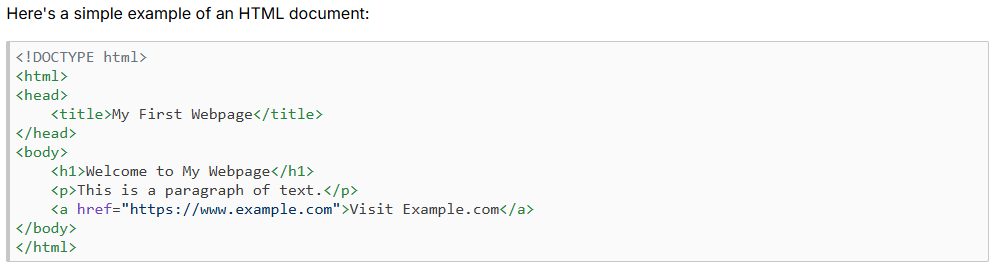
\includegraphics[width=\columnwidth]{figures/webdev-moodle.png}
\caption[WebDev lecture notes in Moodle]{An HTML example from the converted WebDev lecture notes in Moodle. Code is escaped and highlighted, so the example's tags appear as code.}
\label{fig:webdev_result}
\end{figure}

\subsection{Golden Tests}
\label{sec:ev_golden}

Whether a conversion is correct mostly depends on how the package looks in a player, which a unit
test cannot check.
Moreover, a chapter is a large JSON document, and after a change to the renderer the relevant
question is usually whether anything else changed, not whether a single field has a certain value.
The converter is therefore tested with \emph{golden cases}.
Each case is a small folder of Markdown files with a description of how to convert it.
The generated output, that is, the chapter JSON, the package metadata, the warnings, and the packed
images, is committed to version control next to it.
Running the tests writes the output of every case again, so the diff in version control is the
test result.
There is no comparison of expected and actual values and no pass or fail.
Every change in the output has to be reviewed, and if it is intended, it is committed together with
the change to the code.
For this comparison to be useful, the same input must always produce the same output.
Since every block carries a randomly generated identifier, all random values are taken from a single
source that returns a fixed sequence during the tests.
The corpus currently contains 128 cases covering every part of the conversion and merge.

\subsection{Conversion Time}
\label{sec:ev_time}

To determine how long a conversion takes, measurements were conducted on the 12-chapter WebDev corpus and each of the 128 golden cases separately.
They were taken on an AMD Ryzen 7 2700X with 32 GiB of RAM, running Windows 11 Pro and
Oracle Java 19.0.1.
For the warm-JVM measurements, every input was processed three times before ten recorded repetitions.
For comparison, a further ten CLI runs each started a new JVM\@.

\autoref{tab:conversion_time} reports means and sample standard deviations.
A complete conversion includes reading the local input, parsing, rendering, serializing the content,
and creating the package with its bundled libraries.
The parsing and rendering call was also measured separately on the same input.
An additional run measured the consecutive stages of conversion to identify the source of the
time difference.
The fresh CLI runs additionally include JVM startup and delivery of the output file.

\begin{table}[htbp]
\centering
\begin{tabular}{@{}lr@{}}
\toprule
Measurement & Time in ms, mean $\pm$ SD \\
\midrule
WebDev, complete conversion, warm JVM & $375.0 \pm 13.6$ \\
WebDev, parsing and rendering & $33.6 \pm 3.2$ \\
WebDev, packaging alone & $324.0 \pm 14.8$ \\
WebDev, fresh CLI process & $1801.3 \pm 22.2$ \\
\bottomrule
\end{tabular}
\caption[Conversion times for the WebDev lecture notes]{Conversion times for the WebDev lecture notes, with ten recorded repetitions per measurement.}
\label{tab:conversion_time}
\end{table}

The book can be regenerated in under two seconds on this machine, including JVM startup.
Most of the difference between parsing and rendering and a complete conversion comes from
packaging, which takes about 324 ms on its own.
Every conversion includes the same H5P libraries, even for a book containing only a few paragraphs.
For these inputs, packaging overshadows the differences in parsing and rendering.
The content's length and complexity therefore have only a small effect on total conversion time.

The golden cases were also timed individually to identify relatively expensive inputs.
Their mean complete conversion times range from 301 to 341 ms.
The much smaller parsing and rendering times in \autoref{tab:golden_time} again show how strongly the
common packaging work affects this comparison.
The \code{kitchen-sink} case, which comprises all the converter's supported features, takes the longest to parse and render, followed by several
image cases.

\begin{table}[H]
\centering
\small
\begin{tabular}{@{}lrr@{}}
\toprule
Golden Case & Parsing and Rendering & Complete Conversion \\
 & \multicolumn{2}{c}{Time in ms, mean $\pm$ SD} \\
\midrule
\code{kitchen-sink} & $8.3 \pm 1.3$ & $322.8 \pm 14.6$ \\
\code{image-paths} & $5.8 \pm 0.7$ & $311.5 \pm 11.4$ \\
\code{image-data-uri} & $4.3 \pm 0.5$ & $316.1 \pm 12.0$ \\
\code{image-shared-across-chapters} & $3.8 \pm 0.7$ & $309.3 \pm 10.8$ \\
\code{link-md-crosschapter} & $3.6 \pm 0.5$ & $318.4 \pm 30.5$ \\
\bottomrule
\end{tabular}
\caption[Golden cases with the longest parsing and rendering times]{The five golden cases with the longest mean parsing and rendering times, with ten recorded repetitions each.}
\label{tab:golden_time}
\end{table}

The 22 merge cases additionally measured merging after conversion.
Their mean merge times range from 324 to 360 ms; the combined \code{merge-kitchen-sink} case
requires $338.1 \pm 19.4$ ms.
This time includes reading both packages, alignment, and rewriting the output archive.

\newpage
\section{Related Work}
\label{sec:related_work}

To the author's knowledge, no existing tool converts Markdown into an H5P Interactive Book.
Three groups of existing work are related to it.
General document converters could have been extended instead of developing a separate converter.
Plain-text question formats that Moodle already imports offer an alternative to the question extension.
Finally, other H5P content types could have served as the target instead of Interactive Book.

\paragraph{Document Converters.}
Pandoc~\cite{Pandoc} is a general-purpose document converter.
It reads several Markdown dialects and writes dozens of output formats.
A new output format for Pandoc is a writer that works on its document model, so an H5P writer could
have built on a mature parser and a complete model of the input.

For PDF input, a converter into H5P already exists.
\code{pdf\_to\_h5p\_converter} renders every page of a PDF as an image and turns each image into a
slide of a Course Presentation~\cite{Anandh:PdfToH5P}.
Rendering to images would have been possible here as well and much simpler, since only images are
emitted and the constraints on HTML and block placement do not arise.
However, text in an image cannot be searched, selected, resized, or read by a screen reader. It cannot
contain links or questions, and it cannot be edited in the H5P editor, which rules out the editing cycle supported by the merge feature.
The two tools thus represent opposite choices: preserving the appearance of the source or
preserving its structure.

\paragraph{Plain-Text Question Formats.}
If only questions are needed, Moodle can already import them from plain text.
The GIFT format~\cite{Moodle:GIFT} describes a question and its answers in a line-based syntax with
curly braces, and the Aiken format~\cite{Moodle:Aiken} is a stricter format for multiple-choice questions
with lettered answers.
In either case, the questions are imported into the question bank through Moodle's import page~\cite{Moodle:ImportQuestions}.
The converter's own question syntax follows a similar approach but is simpler than either format.

\paragraph{Other H5P Content Types.}
Besides Interactive Book, other H5P content types could have served as the target.
Course Presentation divides content into slides, but a slide is a fixed-size area on which every
element is positioned absolutely.
Text longer than a slide has to be split by hand, so a chapter of
lecture notes does not fit this model.
Page, by contrast, is a single column of content corresponding to one Markdown file, but a book of several files would
become several unrelated pages without navigation between them.
Question Set is a sequence of questions without room for text.
Interactive Book matches the structure of a folder of Markdown files: each file becomes a chapter,
content flows down a column instead of being positioned, and the reader gets a table of contents and
a progress indicator.
Its chapters also accept the layout and interactive content types needed for pseudo-tables and the
editing cycle.
Choosing Interactive Book determined most of the converter's constraints, since the
accepted content types and their \code{semantics.json} define what a Text block may contain.

\newpage
\section{Limitations and Future Work}
\label{sec:limitations}

A successful conversion does not preserve every aspect of the source.
Some differences follow from the content types and HTML that H5P accepts; others follow from the
converter's treatment of Markdown.
\autoref{tab:limitations} summarizes the main approximations and losses.

\subsection{Approximations and Information Loss}
\label{sec:lm_conversion}

\begin{table}[H]
\centering
\small
\begin{tabular}{@{}>{\raggedright\arraybackslash}p{0.23\columnwidth}>{\raggedright\arraybackslash}p{0.73\columnwidth}@{}}
\toprule
Construct & Limitation or Approximation \\
\midrule
Headings and lists & Headings are shifted down one level and clamped at \code{h3}. Tight lists receive the spacing of loose lists. \\
\addlinespace[2pt]
Quotes and inline formatting & Block quotes and alerts become shaded boxes, inserted text receives a green background, and task list checkboxes become characters. \\
\addlinespace[2pt]
Image placement & Images become separate content blocks, interrupting surrounding lists, quotes, or footnotes. \\
\addlinespace[2pt]
Image size & Image blocks have a width attribute, but it is ignored: images occupy the full width of their column. Markdown image size attributes therefore have no effect. \\
\addlinespace[2pt]
Image formats and availability & Unsupported formats, including SVG, and unavailable images are omitted with a warning. \\
\addlinespace[2pt]
Tables with images & Tables with up to four columns become pseudo-tables. Wider tables retain placeholders and place the images below the table. \\
\addlinespace[2pt]
Footnotes & References use bracketed numbers, and the notes form an ordered list at the end of the chapter. \\
\addlinespace[2pt]
Links & Links to other chapters become textual references. Links to Markdown files outside the book lose their destination. \\
\addlinespace[2pt]
Raw HTML & Tags and styles remain subject to the platform's restrictions. Hand-written anchors and links are not rewritten and may therefore collide with generated ids or target the wrong frame. \\
\addlinespace[2pt]
Code and questions & Unknown code languages remain uncolored. Malformed question blocks fall back to code with a warning. \\
\addlinespace[2pt]
Formulas in tables & An unescaped vertical bar splits a table cell before formula parsing. Authors must write \code{\textbackslash|} or \code{\textbackslash{}mid} instead. \\
\addlinespace[2pt]
Metadata & YAML front matter is discarded, and chapter titles derived from file names are not capitalized automatically. \\
\bottomrule
\end{tabular}
\caption[Approximations and information loss]{The main approximations and information loss during conversion. Warnings identify unsupported input, but visual inspection in the player remains necessary.}
\label{tab:limitations}
\end{table}

\subsection{Deployment and Merge Limitations}
\label{sec:lm_platform}

Formulas require the \code{H5P.MathDisplay} add-on on the target site.
The first upload also requires permission to install any bundled libraries that the site does not
already provide.
These requirements cannot be satisfied by the package alone.

Beyond these deployment requirements, the merge can misplace additions when generated blocks are reordered or closely resemble one another.
In addition, generated blocks deleted in H5P reappear after merging, since Markdown remains their source.
Library versions are adjusted without running the libraries' migrations, so these changes produce a
warning.

\subsection{Future Work}
\label{sec:lm_future}

The question syntax could be extended with further question types,
such as fill-in-the-blank or true/false questions.
Each would need a readable fence syntax and a renderer for the corresponding H5P library.
The existing placement mechanism could then handle the resulting blocks.

Packaging could also include only the libraries a book actually uses.
This would reduce package size and the repeated archive work,
but the merge would also need to account for the changing set of libraries.

Finally, automatic rebuilds could run the CLI in a repository's CI pipeline and publish the resulting
package as a build artifact after each change.
Uploading it to Moodle, however, would remain a manual step.

\newpage
\section{Conclusion}
\label{sec:conclusions}

Lecture notes are comfortable to write in Markdown and comfortable to read as H5P content in Moodle.
This thesis presented md2h5p, a converter that turns a folder of Markdown files, a Git
repository, or uploaded files into an Interactive Book package.
Every file becomes a chapter. Text, formatting, images, tables, links, footnotes, and code are
carried over.
Where the target cannot represent a construct, the converter replaces it in a defined way and issues
a warning.
A conversion always produces a book, and its warnings list what the author has to check.

Most of the work follows from what the target does not accept.
The text of an H5P block passes through a sanitizer that keeps a short list of tags and silently removes all
others.
This list is defined per library but is not documented.
The first contribution of this thesis is therefore this list, derived from the implementation and given in
\autoref{tab:allowed}.
Block quotes, deep headings, inserted text, and code boxes are replaced by substitutes built from the
few properties that survive.
Images and tables, in contrast, cannot be markup and become separate content blocks.
Where such a block is placed inside a list, a quote, a footnote, or a table cell is decided by a stack
of render contexts, in which each enclosing construct defines its own behavior.
A table containing an image is rebuilt as a pseudo-table.
Links within a chapter use anchors with ids that are unique across the book.
Links to other chapters, however, are not possible, because the required identifier is assigned by the
platform's database.
Two additions go beyond plain Markdown.
A question syntax uses the info string of a fenced code block as its extension point and remains
valid Markdown in other tools.
A merge combines a new conversion with a package that was edited in H5P, so a book can be extended in H5P
and still regenerated from its source.

Lecturers can keep writing in Markdown, with version control, and no longer have to transfer the
material by hand after every change.
At the same time, what they add in the H5P editor is kept at the next conversion.
Students, in turn, get content that is embedded in their platform, with navigation and progress tracking and
without additional software.

Most of what this thesis states about the platform was derived from its source code, since the
documentation does not cover it.
A design log kept during development records each encountered issue and every decision together with
any rejected alternatives.
Reading the implementation is therefore a starting point for a converter that has to meet an
undocumented contract, while testing on the real platform is necessary to confirm it.

\newpage
\listoftables
\listoffigures
\lstlistoflistings

\bibliographystyle{habbrv}
\clearpage
\phantomsection
\addcontentsline{toc}{section}{\refname}
\label{sec:literature}
\begingroup
\raggedright
\bibliography{bib}  % bib.bib is the name of the Bibliography in this case
\endgroup

\newpage

\end{document}
